\chapter{Úvod}

Robotika je dnes důležitou technologickou oblastí a většina výrobních procesů je automatizována právě za pomocí různých robotických ramen. Navíc dnešní technologie dovolují i~vývoj pokročilých kráčejících robotů, využitelných pro práci v nebezpečných, nepřístupných a náročných terénech.

Díky dostupnosti a cenám drobné modelářské elektroniky je dnes na světě čím dál více nadšenců do této oblasti. Mnoho začátečníků si pro vyzkoušení koupí sadu s odlišnými elektronickými díly - může se jednat o senzory, tlačítka, displaye, malé elektromotory~apod. Po vyzkoušení těchto součástek zjistí, že ho některý typ dílů zaujal více a chtěl by s ním zpracovat nějaký projekt. V případě, že jej zaujmou právě díly, které se mechanicky pohybují, zaujme ho dost možná zrovna robotika. Právě tato práce poskytuje přehled o~tom, co~obnáší návrh a sestavení menších kráčejících robotů.

Cílem této práce bylo nastudování dostupných prostředků vhodných pro sestavení vlastního zařízení využívajícího modelářská serva, navrhnout takové zařízení a sestavit jej. Jako toto zařízení byl v práci zvolen kráčející robot.

Téma spojené s roboty jsem si vybral za účelem vytvoření něčeho, co se skládá i~z~fyzické části a nejedná se tak jenom o program v počítači. Kromě toho se o tuto oblast zajímám delší dobu.

Kapitola \ref{chapterleggedRobots} se zabývá jednotlivými typy kráčejících robotů a způsoby jejich pohybu. V~této kapitole jsou také popsána některá existující řešení daných typů robotů. V kapitole~\ref{chaptertechnologies} jsou popsány existující komponenty využitelné k dosažení výsledku této práce. Analýza současně dostupných technologií spolu s návrhem a specifikací řešení je popsána v kapitole~\ref{chapteranalysis}. Kapitola~\ref{chapterresult} obsahuje popis důležitých částí a výsledků práce. Na konci této kapitoly jsou uvedeny výsledky experimentů s vytvořeným robotem.


%======== Legged robots
\chapter{Existující řešení kráčejících robotů}
\label{chapterleggedRobots}
V této kapitole se nachází základní popis a důležité vlastnosti dvou a více nohých kráčejících robotů. Jelikož tato práce není encyklopedickým přehledem a její rozsah je omezený, u jednotlivých typů robotů se popisují pouze jejich klíčové vlastnosti, vybrané způsoby pohybu, případně konkrétní řešení robota.


V minulých letech se výzkum kráčejících robotů rychle rozšiřoval. Jak uvádí D. J. Todd ve své knize \cite{WalkingMachines}, v případě kráčejících robotů lze koordinovat pohyb velkého množství kloubů pomocí počítače, což zajišťuje plynulý pohyb různorodým terénem. Díky moderním technologiím mohou být tyto řídící počítače umístěny i v malých strojích a robotech.

Jedním z důvodů vývoje kráčejících strojů je zájem o samotnou lokomoci nohou. Pokud je ovšem účelem doprava, je třeba prokázat, že jsou nohy lepší než kola nebo pásy. Dle knihy \cite{WalkingMachines} mohou být výhody kráčejících robotů shrnuty do několika bodů:
\begin{itemize}
    \item Možnost překročení překážek a chůze po schodech.
    \item Kráčející roboti umí dosahovat plynulého pohybu i po hrbolatém terénu.
    \item V principu mohou tito roboti přenášet náklad přes rozbitý terén nebo široké propasti.
    \item Končetiny poškozují povrch méně než pásy nebo spousta kol.
    \item V měkké půdě mají kola problém s hrabáním a mohou uváznout.
\end{itemize}

Z tohoto výčtu vlastností lze určit, zda je pro práci v daném terénu výhodnější použít kráčející roboty, nebo vozidla s pásy, případně koly. Obecně by šlo říci, že v případě hodně členitého a náročného terénu je lepší použít kráčející roboty.


%======== Bipedal
\section{Dvounozí -- bipedal -- roboti}
Konstrukce dvounohých robotů je často inspirována anatomií člověka. Problematikou těchto robotů je jejich špatná stabilita jak v klidu, tak i v pohybu. Udržování rovnováhy u dvounohých robotů lze řešit většími chodidly, jenže ty snižují pohyblivost. Pokročilejší systémy používají akcelerometry nebo gyroskopy k poskytování zpětné vazby a korekci rovnováhy. V literatuře \cite{TwoarmedBipedal} se píše, že v praxi není tak důležité sestavit robota, který nebude padat, ale robota, který se po pádu dokáže zvednout.

\subsection*{Chůze bipedálních robotů}
Podle literatury \cite{TwoarmedBipedal} by měl robot umět řídit své těžiště, aby mohl volně chodit (například robot, popsaný v literatuře \cite{TwoarmedBipedal}, může naklánět kotníky doleva a doprava, díky čemuž dokáže staticky chodit). Pohybová sekvence jednoho cyklu bipedální chůze sestává celkem z osmi fází, jak je ukázáno na obrázku \ref{bipedwalk}. Jeden krok sestává ze čtyř fází: přesunutí váhy na jednu nohu, nadzvednutí nohy, posun nohy dopředu a došlápnutí.

\begin{figure}[hbt]
	\centering
	\includegraphics[width=0.9\textwidth]{obrazky-figures/bipedwalk.png}
	\caption{Chůze dvounohého robota \cite{TwoarmedBipedal}}
	\label{bipedwalk}
\end{figure}

\subsection*{ROBOTIS MINI}
ROBOTIS MINI je stavebnice dvounohého robota od firmy ROBOTIS. Stavebnice obsahuje všechny díly ke kompletnímu sestavení funkčního robota. Dle specifikací v manuálu~\cite{RobotisMini} je vybaven deskou OpenCM9.04-C, s 32bitovým procesorem ARM Cortex-M3 a servy Dynamixel XL-320. Tato serva mají vestavěný procesor a poskytují zpětnou vazbu polohy, teploty nebo točivé síly. Napájení je zajištěno dvěma Li-ion bateriemi. Robota lze doplnit o různé periferie jako například LED modul, tepoloměr, gyroskop nebo magnetický senzor. Zdrojové kódy i 3D modely dílů jsou open source a volně dostupné ke stažení z online manuálu~\cite{RobotisMini}. Díky tomuto podrobně zpracovanému manuálu a hotové ovládací aplikaci je kit ROBOTIS MINI vhodný i pro začátečníky. Pokročilejší uživatelé si pak mohou vytisknout upravnené díly nebo doplnit robota různými senzory  a přizpůsobit řídící aplikaci.

\begin{figure}[hbt]
	\centering
	\includegraphics[width=0.29\textwidth]{obrazky-figures/robotismini.png}
	\caption[robotis]{Sestavený robot ROBOTIS MINI \cite{RobotisMini}}
	\label{robotismini}
\end{figure}


%======== Quadruped 
\section{Čtyřnozí -- quadruped -- roboti}
Při srovnání s různými typy kráčejících robotů mají čtyřnozí roboti minimální počet nohou zajištující statickou chůzi a přijatelnou stabilitu. Podle literatury \cite{QuadrupedTitan} lze čtyřnohé roboty rozdělit na základě konfigurace nohou do dvou skupin: savčí typ a hmyzí typ. Jak ukazuje obrázek \ref{quadType}, u savčího typu je základní poloha nohou svislá, kdežto hmyzí typ má první segment nohy umístěn vodorovně a druhý i třetí segment vertikálně.

Jak uvádí literatura \cite{QuadrupedTitan}, čtyřnohý robot savčího typu má několik výhod. Dokáže se~pohybovat rychleji než hmyzí typ a povahou konstrukce nohou je v každém kloubu vyžadován menší točivý moment, zvláště když robot stojí. Savčí typ je také mnohem užší a dokáže procházet stísněnými prostory. Na druhou stranu je hmyzí typ vysoce stabilní díky nízko položenému těžišti a širokému rozložení nohou. Hmyzí typ může navíc při pohybu použít své tělo jako pátou nohu v závislosti na terénu.

\begin{figure}[hbt]
	\centering
	\includegraphics[width=0.5\textwidth]{obrazky-figures/quadTypes.png}
	\caption{Základní typy čtyřnohých robotů \cite{QuadrupedTitan}}
	\label{quadType}
\end{figure}

\subsection*{Algoritmus chůze čtyřnohých robotů použitelný pro oba typy}
Tento typ chůze je vhodný pro pomalý a stabilní pohyb, jelikož je při každém kroku zdvižena právě jedna noha a ostatní tři podpírají tělo. Těžiště robota se nachází vždy nad polygonem tvořeným podpěrnými nohami. Dle článku o chůzi čtyřnohých robotů \cite{QuadrupedWalk} může být šest možných sekvencí nohou, které splňují podmínku, že se těžiště nachází vždy nad polygonem, přičemž se robot pohybuje rovně. Jedna možná sekvence je zobrazena na obrázku~\ref{quadWalk}.

\begin{figure}[hbt]
	\centering
	\includegraphics[width=0.76\textwidth]{obrazky-figures/quadWalk.png}
	\caption{Jeden cyklus algoritmu chůze čtyřnohých robotů \cite{QuadrupedWalk}}
	\label{quadWalk}
\end{figure}

\subsection*{Klus čtyřnohých robotů savčího typu}
S tímto typem pohybu je možné dosahovat vyšších rychlostí za cenu nižší stability. Jak~uvádí článek o pohybu čtyřnohých robotů \cite{QuadrupedTrot}, v jednom okamžiku slouží dvě protější nohy jako podpěra a další dvě jsou zdviženy. Na konci každého kroku se funkce dvojic protějších nohou prohodí. Protože v jeden moment stojí robot pouze na dvou nohách, vzniká zde neřízený stupeň volnosti náklonu těla. Tento stupeň volnosti je nutno řídit pomocí správného naplánování trajektorie pro každou zvedanou nohu.

\subsection*{Boston Dynamics Spot}
Spot je nejnovější čtyřnohý robot připomínající psa od společnosti Boston Dynamics. Článek zabývající se vývojem čtyřnohých robotů \cite{QuadrupedSpot} uvádí, že se jedná o nový přístup k~dynamickému řízení robotů ve srovnání s předchozími modely od této společnosti (robot BigDog nebo LS3). Spot měří přibližně $110cm$ x $50cm$ x $84cm$ (délka x šířka x výška) a dokáže běžet rychlostí $5,76km/h$. Jeho celková hmotnost dosahuje $30kg$ a je schopen nést náklad o váze $14kg$. Robota napájí baterie a všechny jeho klouby jsou ovládány elektrickými aktuátory (akčními členy). Konstrukce v kombinaci s vestavěnými počítači umožňuje chůzi i~klus do všech směrů, sestup nebo výstup schodů, pohyb v nerovném terénu, vyvažování a~přizpůsobení se vnějším vlivům.

Spot má zabudovaný systém 3D vidění se simultánní lokalizací a mapováním (SLAM).  Tento systém poskytuje informace, pomocí nichž robot vnímá své okolí a umí se vyhýbat překážkám. Vestavěné počítače se starají o lokomoci a navigaci. Řízení robota probíhá dálkově operátorem, přičemž některé úkony jsou prováděny autonomně. Dle literatury \cite{QuadrupedSpot} se Spot stal nejlehčím robotem, který je vhodný pro vnitřní i venkovní provoz.

\begin{figure}[hbt]
	\centering
	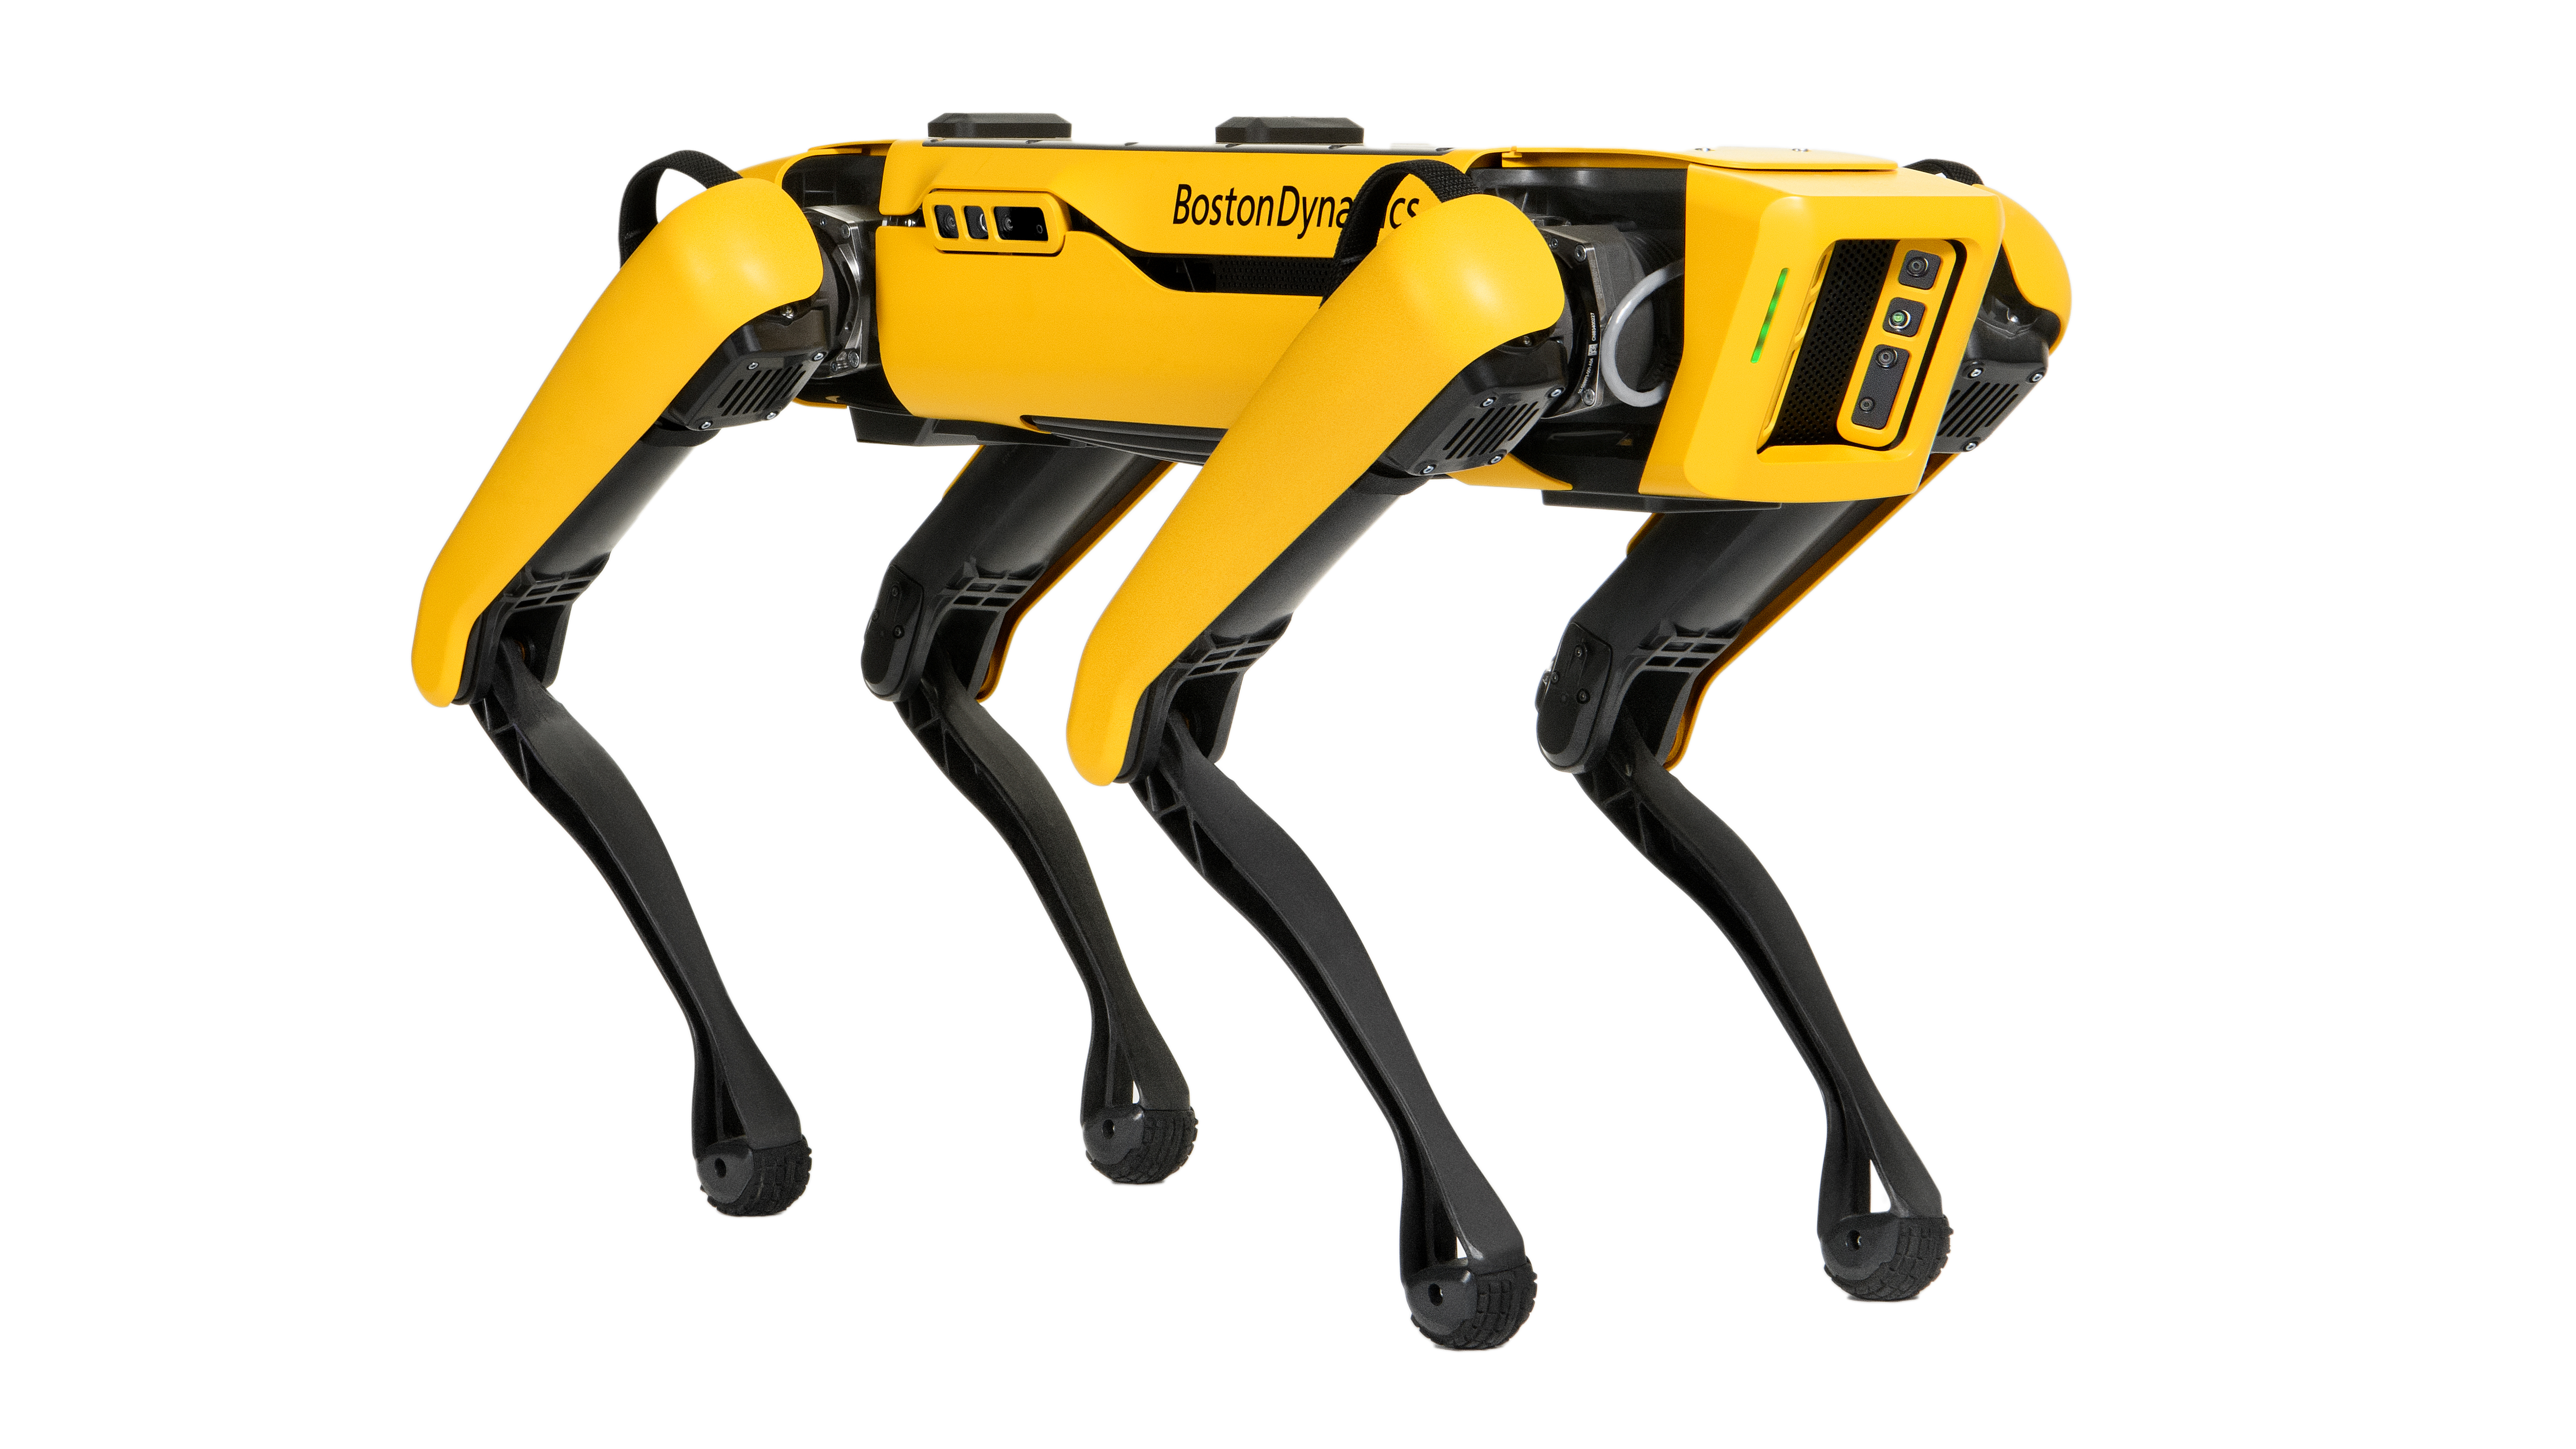
\includegraphics[width=0.6\textwidth]{obrazky-figures/spot.png}
	\caption[spot]{Spot od Boston Dynamics\footnotemark}
	\label{quadSpot}
\end{figure}
\footnotetext{Obrázek převzat z webové stránky https://www.bostondynamics.com/spot}


%======== Hexapod
\section{Šestinozí roboti -- hexapodi}
Konstrukce hexapodů se inspiruje mechanikou hmyzu. Počet šesti nohou je ideální pro dobrou stabilitu s nepříliš složitou konstrukcí. Vzhled a tvar hexapodů může být různý, ale obecně je lze rozdělit podle tvaru těla na hexagonální (kruhové) a obdélníkové. Obdélníkový hexapod má tělo ve tvaru obdélníku s končetinami rozmístěnými symetricky po jeho delších stranách. Hexagonální robot má nohy rozmístěny rovnoměrně po obvodu svého kruhového těla. V článku o lokomoci hexapodů \cite{HexapodSymetric} se zmiňuje, že podle výzkumů je obdélníkové tělo zvýhodněno při přímé chůzi dopředu nebo chůzi do stran. Nicméně pro otáčení vyžaduje speciální model pohybu. Hexagonální tvar těla poskytuje lepší výsledky v určitých ohledech. Hexapodi s tímto tvarem mohou mít mnoho druhů chůze a snadno měnit její směr.

\subsection*{Design končetin a kinematika}
Končetiny hexapodů byly navrženy tak, aby optimalizovaly pohyby jedné nebo více končetin současně. Současný koordinovaný pohyb více končetin je důležitý jak pro samotnou chůzi, tak i pro zdolávání různých překážek nebo změnu výšky robota pro manévrování v~různých prostředích. Jak uvádí literatura \cite{HexapodDesign}, končetina hexapoda byla navržena jako třídílná struktura. Podle analogie s biologickými organismy se tyto části nazývají coxa (kyčel), femur (stehno) a tibia (holeň). Na obrázku \ref{hexleg} je ukázáno, že coxa spojuje nohu s tělem hexapoda ve vodorovné ose a femur spojuje coxu a tibii v ose svislé. Každá noha má tedy 3 stupně volnosti, což dává hexapodovi celkem 18 stupňů volnosti.

\begin{figure}[hbt]
	\centering
	\includegraphics[width=0.4\textwidth]{obrazky-figures/hexleg.png}
	\caption{Struktura končetiny robota hmyzího typu \cite{HexapodDesign}}
	\label{hexleg}
\end{figure}

Pro správnou koordinaci nohou je třeba použití kinematiky. V robotice se bere v potaz přímá kinematika a inverzní kinematika. V případě přímé kinematiky jsou známy úhly jednotlivých kloubů a vypočítávají se souřadnice koncového bodu. Naopak inverzní kinematikou lze podle známých souřadnic koncového bodu vypočítat odpovídající úhly kloubů.

\subsubsection*{Přímá kinematika končetiny}
Kinematický řetězec mechanizmu nohy se třemi rotačními klouby je spolu s označením souřadnic a symbolů zobrazen na obrázku \ref{hexkin}. Geometrický model z dokumentu o kinematice robotů \cite{HexapodKinematics} je formulován mezi pohyblivým souřadným systémem $O_i(x_i, y_i, z_i), i = 0...3$ spojeným se základnou nohy, a pevným globálním souřadným systémem $O_G(x_G, y_G, z_G)$. Tento vztah se řídí přímým geometrickým modelem Denavit-Hartenberg. Pro určení celkové transformace od coxy ke špičce nohy lze použít rovnice:
\begin{equation}
\boldsymbol{T}_{coxa}^{tip}=\boldsymbol{T}_{coxa}^{femur}\boldsymbol{T}_{femur}^{tibia}\boldsymbol{T}_{tibia}^{tip}
\end{equation}



Výsledné souřadnice špičky nohy lze vypočítat podle rovnic z literatury \cite{HexapodKinematics}:

\begin{equation} \label{eqDirKin}
\begin{split}
x & =[l_{1}+l_{2}\cos\theta_{2}+l_{3}\cos(\theta_{2}-\theta_{3})]\cos\theta_{1} \\
y & =[l_{1}+l_{2}\cos\theta_{2}+l_{3}\cos(\theta_{2}-\theta_{3})]\sin\theta_{1} \\
z & =d_{1}+l_{2}\sin\theta_{2}+l_{3}\sin(\theta_{2}-\theta_{3}) 
\end{split}
\end{equation}

Význam jednotlivých symbolů v rovnicích \eqref{eqDirKin}: $d_1$ -- vzdálenost kloubu coxy od souřadnice $O_G$ v ose Z; $l_i$ -- délka segmentu nohy (1 -- coxa, 2 -- femur, 3 -- tibia); $\theta_i$ -- úhel kloubu (1 -- coxa, 2 -- femur, 3 -- tibia).

\begin{figure}[hbt]
	\centering
	\includegraphics[width=0.5\textwidth]{obrazky-figures/hexkinematics.png}
	\caption{Model končetiny s vyznačenými souřadnicemi a proměnnými \cite{HexapodKinematics}}
	\label{hexkin}
\end{figure}

\subsubsection*{Inverzní kinematika končetiny}
Inverzní kinematika je v případě hexapodů používanější a přináší přirozenější pohyb robota. Jednotlivých úhlů kloubů $\theta_1$, $\theta_2$ a $\theta_3$ (coxa, femur a tibia) lze dosáhnout pomocí výsledných vzorců \eqref{eqInvKin} uvedených v literatuře \cite{HexapodKinematics}:

\begin{equation} \label{eqInvKin}
\begin{split}
& \theta_{1}=\begin{cases} arctg\left(\frac{y}{x}\right)+\pi, x < 0 \\ arctg\left(\frac{y}{x}\right), jinak \end{cases} \\
& \theta_{2}=arccos\frac{l_{2}^{2}+x^{\prime 2}+y^{\prime 2}-l_{3}^{2}}{2l_{2}\sqrt{(x^{\prime 2}+y^{\prime 2})}}+arctg\frac{y_{3}}{x_{3}} \\
& \theta_{3}=\pi-arccos\frac{l_{3}^{2}+l_{2}^{2}-(x^{\prime 2}+y^{\prime 2})}{2l_{2}l_{3}}
\end{split}
\end{equation}

Nové proměnné $x$, $y$ představují souřadnice špičky nohy v souřadnicovém systému nohy ($x_G$ a $z_G$) a proměnné $x^{\prime}$, $y^{\prime}$ souřadnice špičky nohy v souřadnicovém systému coxy ($x_G$~a~$y_G$).


\subsection*{Tripedální chůze ``3+3''} \label{sectripodgait}
Při tripedální chůzi se nohy hexapoda rozdělí do dvou skupin po třech, podle obrázku \ref{tripodgait} na A, C, E (levá přední noha, levá zadní a pravá prostřední) a B, D, F (levá prostřední, pravá přední a pravá zadní). Jedna skupina nohou podepírá tělo robota a posunuje jej dopředu. Druhá skupina nohou je zdvižená a pohybuje se dopředu. Na obrázku \ref{tripodgait} je vyznačena podpůrná skupina nohou zeleně a zdvižené nohy červeně. V každé periodě chůze se robot posune o dva kroky. V článku o chůzi hexapodů \cite{HexapodSymetric} je uvedeno, že doba styku se zemí je 1/2 periody. Tripedální chůze představuje optimální stabilitu i rychlost pro šestinohé roboty.

\begin{figure}[hbt]
	\centering
	\includegraphics[width=0.8\textwidth]{obrazky-figures/tripodgait.png}
	\caption{Základní perioda tripedální chůze hmyzího typu}
	\label{tripodgait}
\end{figure}

Tripedální chůze má dva typy podle směru chůze. V literatuře \cite{HexapodSymetric} jsou tyto typy označeny jako savčí a hmyzí. Při savčí chůzi se nohy pohybují primárně ve svislé rovině, což vede k minimálnímu otáčení kloubů coxy. Při tomto typu chůze se robot pohybuje jako krab, tedy zleva doprava a zprava doleva. Na druhou stranu je hmyzí chůze využívána především k pohybu dopředu a dozadu, přičemž jsou klouby coxy namáhány nejvíce. Pro~realizaci hmyzí chůze musí mít každá noha robota tři stupně volnosti.

\subsection*{Chůze ``4+2''}
Pro chůzi ``4+2'' jsou nohy rozděleny celkem do tří skupin po dvou. Tělo podepírají vždy čtyři nohy (dvě skupiny) stojící na zemi a zbylé dvě nohy se zdvižené pohybují dopředu. Jedna perioda se skládá ze tří kroků, ale robot se posune pouze o jeden krok vpřed. Doba styku se zemí jsou 2/3 periody. Literatura \cite{HexapodSymetric} uvádí, že tento typ chůze je do jisté míry odolný vůči chybám, protože při poškození jedné nohy zůstávají další tři, které podepírají tělo.

\begin{figure}[hbt]
	\centering
	\includegraphics[width=1\textwidth]{obrazky-figures/42gait.png}
	\caption{Perioda chůze ``4+2''}
	\label{42gait}
\end{figure}

\subsection*{Vlnová chůze ``5+1''}
Při vlnové chůzi je v jednu chvíli zdvihána a posunována dopředu jen jedna noha. Ostatní nohy podepírají tělo a pomalu jím pohybují ve směru chůze. Vlnová chůze je nejstabilnější a nejlépe odolná vůči chybám. Nicméně je pomalá, protože robot je ve styku se zemí~5/6 periody. Podle literatury \cite{HexapodSymetric} se tato chůze používá pro speciální případy pohybu, například otáčení tělem nebo zdolávání náročného terénu a překážek.

\subsection*{PhantomX AX Mark-III}
Jedná se o třetí revizi populárního hexapoda od firmy Interbotix Labs. PhantomX~AX Mark-III je dostupný ve formě stavebnice v několika variantách \cite{PhantomX}. Tato sada se stala jednou z nejpokročilejších robotických platforem vhodných pro výzkumné pracovníky i pro nadšence do robotiky.

Kompletně hliníková konstrukce přináší vysokou odolnost \cite{PhantomX}. Pro otáčení pohyblivých částí (kloubů) jsou použita výkonná serva DYNAMIXEL AX-12A (případně AX-18A), přičemž každá končetina má tři stupně volnosti. Chod hexapoda řídí deska ArbotiX Robocontroller, která je kompatibilní s Arduinem. O napájení vešekeré elektroniky robota se~stará tříčlánková Li-Pol baterie s kapacitou 4500mAh. Pro robota jsou k dispozici různé manuály, ukázkové open source programy i kompletní řídicí aplikace.

\begin{figure}[hbt]
	\centering
	\includegraphics[width=0.6\textwidth]{obrazky-figures/hex-a.jpg}
	\caption[phantom]{Sestavený PhantomX AX Mark-III \cite{PhantomX}}
	\label{hexphantom}
\end{figure}


%======== Eight-legged
\section{Osminozí roboti - octapodi}
Oproti předchozím typům robotů přinášejí osminozí roboti nejlepší stabilitu při maximální rychlosti chůze. Dle literatury \cite{ArachnidRobot} jsou navíc méně náchylní k neschopnosti dalšího pohybu při selhání aktuátorů - mohou udržovat stabilitu a téměř plnou rychlost i při poruše jedné až dvou končetin. Nicméně stavba a údržba osminohých robotů je složitější díky více pohyblivým částem. Osminozí roboti se svou konstrukcí těla i končetin dost podobají šestinohým robotům, takže i algoritmy jejich chůze jsou si podobné. Mezi komerční řešení osminohých robotů patří například robot T8X od firmy Robugtix \cite{t8x}.



%======== Technologies
\chapter{Technologické prostředky ke stavbě malých robotů}
\label{chaptertechnologies}

Tato kapitola se zabývá popisem momentálně dostupných elektronických komponent, možností bezdrátové komunikace a způsobu výroby dílů, což lze využít právě při tvorbě malých robotů. Takových technologických prostředků je velké množství a pro každého robota se může hodit něco jiného. Tato sekce tedy není encyklopedickým přehledem všech dostupných technologií a z důvodu omezeného rozsahu této práce jsou zde popsány technologické prostředky bezprostředně spojeny s touto~prací.


\section{Modelářská serva}

V modelářském časopisu \cite{ServoMagazine} je servo zjednodušeně specifikováno jako motorizovaná převodovka, která se otáčí do určité polohy nebo se pohybuje specifikovanou rychlostí určenou vstupním signálem. Článek o modelářských servech \cite{HobbyServos} přesněji udává, že servo je elektromechanický zpětnovazební systém. Modelářská serva se běžně používají například v dálkově ovládaných letadlech nebo autech a malých robotech. Modelářská serva se vyrábějí v několika provedeních pro různé případy použití: od miniaturních slabých serv s plastovou převodovkou až po silná a odolná serva s větším motorem, kuličkovými ložisky a plně kovovými převody~\cite{HobbyServos}.

\begin{figure}[hbt]
	\centering
	\includegraphics[width=0.3\textwidth]{obrazky-figures/servo1.jpg}
	\caption[servo]{Modelářské servo\footnotemark}
	\label{servo1}
\end{figure}
\footnotetext{Obrázek převzat z: https://www.pololu.com/product-info-merged/3426}

Serva lze obecně rozdělit podle typu použitého elektromotoru na AC serva -- využívají elektromotor na střídavý proud a DC serva -- použitý elektromotor potřebuje stejnosměrný proud. Protože se tato sekce zabývá modelářskými servy, která jsou vybavena elektromotorem na stejnosměrný proud, všechny následující informace se týkají DC serv.

\subsection*{Princip činnosti serva}
Modelářské servo se skládá z těchto čtyř základních částí: stejnosměrný elektromotor, zařízení pro snímání polohy (potenciometr), převodovka a řídící obvod. Dle článku o modelářských servech \cite{HobbyServos} je princip činnosti serva shrnut v následujících větách.

Na vstupní pin serva je přiveden impulz (elektrický pulz proměnné šířky nebo signál pulzně šířkové modulace), který se převádí na vstupní napětí pro řídící integrovaný čip. Toto napětí je porovnáno se zpětnovazebním napětím odvozeným z polohy potenciometru. Potenciometr je přímo spojen s hřídelí serva, díky čemuž dokáže snímat mechanickou polohu hřídele. Chybový zesilovač detekuje, zda existuje rozdíl mezi vstupním a zpětnovazebním napětím. Rozdíl těchto dvou napětí je následně zesílen a aplikován jako vstup do servomotoru. Pokud je výstup zesilovače kladný, motor se točí jedním směrem a pokud záporný, motor se točí opačně. Chod motoru otáčí hřídelí serva a zároveň i potenciometrem tak, aby hřídel dosáhla polohy, jež odpovídá vstupnímu signálu. Po dosažení požadované polohy je zpětnovazební napětí shodné se vstupním napětím a jejich rozdíl je nulový. Nulový rozdíl napětí způsobuje zastavení servomotoru, který dále drží tuto polohu.

\begin{figure}[hbt]
	\centering
	\includegraphics[width=0.6\textwidth]{obrazky-figures/servo-parts-labeled.jpg}
	\caption[servoInternal]{Vnitřní složení modelářského serva\footnotemark}
	\label{servo_internal}
\end{figure}
\footnotetext{Obrázek převzat z: https://cdn.sparkfun.com/assets/custom\_pages/5/6/0/servo-parts-labeled.jpg}

\subsubsection*{Pulzně šířková modulace - PWM}
Digitální signál má dvě polohy: 1 (zapnuto) a 0 (vypnuto). Analogový signál může nabývat libovolné hodnoty od 0 do 1. Podle článku o PWM \cite{servoAnalogIcTips} se s těmito signály zachází v elektronice zcela odlišně, nicméně často je vyžadována práce s oběma typy současně. Analogový vstup se převádí na digitální signál pomocí analogově digitálního převodníku - ADC. Naopak pro řízení analogových zařízení pomocí digitálního výstupu je nutno použít právě PWM. Pomocí PWM lze mikrokontrolerem řídit zařízení, jež na vstupu očekávají analogový signál (například motory s proměnnou rychlostí nebo stmívatelná světla). U tohoto signálu se napětí vysílá v tzv. pulzech. U signálu PWM je klíčová frekvence (doba periody v Hz) a střída (angl. duty cycle) pulzů. Střída představuje v procentech část periody, kdy je signál v poloze logické 1. Průměrné výstupní napětí lze vypočítat vynásobením střídy a~hodnoty napětí v logické 1. Například pokud je střída $50\%$ a napětí v log. 1 má hodnotu $24V$, výstupní napětí bude $24*0,5= 12V$.

\subsection*{Typy serv podle pohybu hřídele a další parametry serv}
Standardní polohově otáčivá serva mohou otáčet hřídelí v rozsahu zhruba 180 stupňů. Jak uvádí modelářský časopis \cite{ServoMagazine}, serva jsou proto vybavena mechanickými zarážkami (často se tato zarážka nachází na výstupním ozubeném kole), aby se zamezilo rotaci mimo rozsah. U některých serv je zase výstupní kolo ozubené pouze z poloviny. 

Pro jiné případy použití existují i kontinuálně otáčivá a lineární serva. Kontinuálně otáčivá serva mají stejný vzhled jako polohově otáčivá, ale liší se interně. Nejsou u nich použity mechanické zarážky a dokážou nepřetržitě otáčet hřídelí v obou směrech. Místo polohy hřídele se u kontinálně otáčivých serv řídí jejich rychlost, která podle modelářského časopisu \cite{ServoMagazine} typicky dosahuje $40$ až $50ot/min$. Lineární servo nabízí více rychlostních stupňů a využívá hřebenový mechanismus pro pohyb z jedné strany na druhou, namísto otáčivého pohybu. Pro řízení lineárního serva se používá stejný signál jako pro standardní servo.

Modelářská serva se také vyrábějí v různých velikostech pro jednotlivé případy užití. Mezi základní velikosti patří serva s označením Micro, Standard a Giant.

Kromě typu otáčení a velikosti se mohou serva lišit v materiálu použitém při výrobě jejich převodovky. Převodovka může být plastová, kovová nebo hybridní. Hybridní slouží jako ochrana motoru před spálením - pokud se páka serva zasekne, plastové ozubené kolečko se ohlodá, díky čemuž se motor může otáčet a nedojde k jeho zničení.

Serva se také dělí na digitální a analogová. Oba typy se řídí stejně z pohledu uživatele, rozdíl je v jejich interní elektronice.



\subsection*{Digitální servo}
V literatuře \cite{DigitalServo} je uvedeno, že digitální servo je stejné jako standardní analogové servo, s výjimkou vestavěného mikroprocesoru, který zpracovává vstupní signál a ovládá motor serva. Digitální serva se tedy fyzicky neliší od těch analogových: mají stejný motor, převodovku i zpětnovazební potenciometr. V čem jsou digitální serva rozdílná, je způsob zpracovávání vstupního signálu a způsob řízení servomotoru. Digitální servo pomocí svého mikroprocesoru aplikuje paramtery na příchozí signál, a následně posílá pulzy tohoto modifikovaného signálu na servomotor. Tímto je optimalizován celkový výkon serva. Mikroprocesor digitálního serva posílá na servomotor pulzy s mnohem vyšší frekvencí. To znamená, že servomotoru přichází až 300 pulzů za sekundu, místo 50. Délka pulzů se snižuje v přímém poměru vzhledem k vyšší frekvenci, což vede k častějšímu zapínání a vypínání servomotoru. Díky těmto vlastnostem má digitální servo skvělou odezvu, minimální odchylku mrtvé zóny (anglicky deadband), rychlejší a plynulejší zrychlení/zpomalení a lépe udrží svou polohu. Dle literatury \cite{DigitalServo} je jedinou nevýhodou digitálního serva jeho vysoká spotřeba elektrické energie.

\subsection*{Standardní/analogové servo}
Analogové servo je vybaveno pouze vlastní logickou deskou, která nemodifikuje vstupní signál. V literatuře \cite{DigitalServo} je napsáno, že v nečinnosti není na servomotor posíláno žádné napájení. Napětí se na servomotor přivádí až tehdy, pokud je přijat vstupní signál pro změnu polohy hřídele nebo pokud na rameno hřídele působí vnější síla. Toto platí i pro digitální servo. V případě analogového serva je napětí na servomotor posíláno v pulzech s konstantní rychlostí 50 pulzů za sekundu. Článek na webové stránce \cite{ServoRadioControlInfo} uvádí, že analogové servo je levnější a má nižší spotřebu elektrické energie. Na druhou stranu má analogové servo pomalejší odezvu, vyšší odchylku mrtvé zóny a slabé držení polohy.

Na obrázku \ref{analogdigital} jsou porovnány pulzy analogového a digitálního signálu. První diagram ukazuje signál, kdy je motor v nečinnosti, na druhém je zobrazen krátký signál -- nízké napětí na servomotoru. Diagram 3 porovnává delší pulz -- vyšší naptětí na motoru.


\begin{figure}[hbt]
	\centering
	\includegraphics[width=0.75\textwidth]{obrazky-figures/analogVdigital.png}
	\caption{Porovnání signálu analogového a digitálního serva \cite{DigitalServo}}
	\label{analogdigital}
\end{figure}

\subsection*{Řízení modelářského serva uživatelem}
Serva mají tři vývody, kterými se připojují k řídící platformě (např. k mikrokotroleru). Dva vývody slouží pro napájení (většina serv lze napájet pomocí napětí $4,6$ -- $6V$). Třetím je posílán vstupní signál. Barvy těchto vodičů se mohou lišit podle výrobce, často se však používá kombinace hnědá (mínus), červená (plus) a oranžová (signálový vodič).

Kromě zapojení napájení je nutné připojit i signálový vodič serva, kde budou posílány pulzy proměnné délky (pro tento účel se často používá PWM). Servo očekává pulz každých $20ms$ a délka pulzu udává požadovanou polohu hřídele. Článek na webové stránce \cite{servoCircuitDigest} uvádí, že výchozí pozici 90° odpovídá pulz o délce $1,5ms$. Pro krajní pozice 0° je aplikován pulz dlouhý $1ms$ a pro 180° bude tento pulz trvat $2ms$. V závislosti na výrobě serva se~délka pulzu pro jednotlivé úhly může lišit. Pro generování signálů PWM a řízení serv jsou dostupné různé knihovny pro jednotlivé řídicí desky.


\subsubsection{Řízení modelářského serva SG90}
Servo SG90 patří mezi nejlevnější a nejrozšířenější modelářská serva. Pro jeho ovládání je potřeba určit střídu odpovídající danému úhlu. Ta lze vypočítat podle vzorce
$$\textit{střída} = \frac{a}{180} * \alpha + b$$
kde $a$ značí střídu odpovídající 180°, $\alpha$ požadovaný úhel, $b$ je střída odpovídající 0°. U~tohoto serva je $a = 10$, $b = 2$ \cite{servoPythonExemplary}.

\begin{figure}[hbt]
	\centering
	\includegraphics[width=0.95\textwidth]{obrazky-figures/servomot1.png}
	\caption[sg90]{Odpovídající poloha serva SG90 pro jednotlivé délky signálu\footnotemark}
	\label{sg90}
\end{figure}
\footnotetext{Obrázek převzat z: http://www.python-exemplary.com/raspi/rgifs/servomot1.png}


\subsection*{Knihovna LedC pro ESP32}
Knihovna LedC je wrapper\footnote{Wrapper - vrstva kódu převádějící existující rozhraní knihovny na jiné kompatibilní rozhraní.} knihovny LED Control pro platformu Arduino (C/C++). Dle dokumentace \cite{servoLEDControl} je knihovna primárně navržena pro ovládání intenzity svitu LED diod, nicméně lze použít i pro generování signálů PWM pro jiné účely, například ovládání serva. Knihovna LedC umožňuje generovat až 16 na sobě nezávislých signálů PWM na tzv.~kanálech. Pro každý kanál lze nastavit frekvenci a rozlišení signálu. Kanál je pak přiřazen na zvolený pin s podporou PWM a tímto pinem se bude vysílat generovaný signál. Délku generovaného pulzu je možné měnit podle potřeby.

Knihovna LED Control má kanály rozděleny do dvou skupin po osmi. Jedna skupina pracuje ve vysokorychlostním režimu. Ten je implementován v hardwaru a nabízí automatickou a bezproblémovou změnu střídy PWM. Druhá skupina kanálů pracuje v režimu nízké rychlosti a střída musí být změněna ovladačem v softwaru, což je pomalejší. Řadič PWM může automaticky plynule zvyšovat nebo snižovat střídu bez jakéhokoli rušení procesoru, takže nezpůsobuje jittering (třes) serva. U knihovny LedC režim zvolit nelze a všechny kanály pracují ve vysokorychlostním režimu.




\section{Platformy pro řízení serv}
Mikrokontrolerů a vývojových desek vhodných pro použití v malých robotech za účelem komunikace a ovládání periferií (například řízení serv, čtení dat ze senzorů) je celá řada a jejich výběr spíše záleží na preferenci uživatele. V této části se vyskytuje popis několika známých platforem.


\subsection*{ESP32}
ESP32 je řada SoC\footnote{System On Chip - čip nebo integrovaný obvod, který obsahuje hned několik částí počítače (obvykle CPU, RAM, I/O porty a paměť ROM)\cite{soc}.} mikrokontrolerů vyvíjených firmou Espressif Systems. Dle datasheetu~\cite{espNet} se jedná o nástupce čipu ESP8266 a je dodáván v jednojádrových i dvoujádrových variantách 32bitového mikroprocesoru Tensilica Xtensa LX6 s integrovanou Wi-Fi (2.4GHz) a Bluetooth (v4.2 + BLE). Procesor pracuje s frekvencí 160 nebo 240MHz a je doplněn koprocesorem s nízkou spotřebou. Čip disponuje 448 KiB ROM (paměť pro bootování a klíčové funkce), 520 KiB SRAM (data a instrukce) a interní FLASH pamětí 0/2/4 MiB podle verze čipu. ESP32 podporuje doplnění o externí QSPI FLASH paměť s kapacitou až 16 MiB.

Konektivita ESP32: 34 programovatelných GPIO pinů s hardwarovou podporou PWM (až 16 kanálů), 12bitový ADC a 8bitový DAC, SPI, I2C, I2S, UART.

ESP32 je dostupný jako samotný čip (např. ESP32-D0WDQ6) nebo PCB modul pro povrchovou montáž -- SMD (např. ESP-WROOM-32). SMD moduly jsou navrženy pro zabudování do finálních produktů, a tak postrádají komponenty, které nejsou vhodné pro finální produkty, např. žádný USB-UART převodník ani programovací/reset tlačítka. Tímto se minimalizuje cena i velikost modulu. Pro účely prototypování a vývoje lze použít některou z dostupných vývojových desek.

Díky velkému množstí open-source zdrojů podporuje ESP32 vývoj různými způsoby (například LUA, MicroPython, C/C++, AT příkazy atd.).

\begin{figure}[hbt]
	\centering
	\includegraphics[width=0.5\textwidth]{obrazky-figures/espdevkit.jpg}
	\caption[esp32board]{Vývojová deska s modulem ESP-WROOM-32\footnotemark}
	\label{esp}
\end{figure}
\footnotetext{Obrázek převzat z: https://rpishop.cz/robotika-a-vzdelavani/1500-esp32-vyvojova-deska.html}

\subsubsection{ESP32 DOIT Devkit V1}
Jedná se o vývojovou desku založenou na modulu ESP-WROOM-32 (s čipem ESP-D0WDQ6). Dle dokumentace \cite{espDevkit} má integrovaný USB-UART převodník CP2102 a 2 tlačítka pro reset nebo uživatelem definované funkce. Všechny I/O piny modulu ESP-WROOM-32 jsou přístupné přes rozšiřující headery a mají logickou úroveň $3,3V$. Na desce se nachází USB konektor pro napájení, programování firmwaru nebo debug UARTu. Zabudovaná FLASH má v tomto případě kapacitu 4MiB.


\subsection*{Arduino Uno R3}
Arduino je open-source platforma založená na snadno použitelném hardwaru a softwaru (Arduino IDE). Desek Arduino je velké množství a právě Uno patří mezi nejznámější.

Uno je deska mikrokontroleru založená na čipu ATmega328P. Ve schématech \cite{arduinoUno} se uvádí, že Uno má k dispozici 14 digitálních vstupně výstupních pinů s logickou úrovní $5V$ (z nichž lze 6 použít jako výstupy PWM), 6 analogových vstupů, podporu I2C, krystal o frekvenci 16MHz, USB připojení pro nahrávání programu, napájecí konektor, záhlaví ICSP a tlačítko reset. Uno je vhodné pro úplné začátečníky díky své odolnosti vůči nesprávnému zacházení -- v nejhorším případě lze vyměnit čip ATmega328P a začít znovu.

\begin{figure}[hbt]
	\centering
	\includegraphics[width=0.5\textwidth]{obrazky-figures/arduino.jpg}
	\caption[arduino]{Arduino Uno R3\footnotemark}
	\label{uno}
\end{figure}
\footnotetext{Obrázek převzat z: https://store.arduino.cc/arduino-uno-rev3}



\subsection*{Raspberry Pi}

Raspberry Pi je série jednodeskových počítačů vyráběných firmou Raspberry Pi Foundation. Od své první verze zveřejněné v roce 2012 bylo vydáno několik různých variant. Originální verze Pi měla jednojádrový procesor s frekvencí 700MHz a pouze 256MB RAM, přičemž poslední model je vybaven čtyřjádrovým procesorem s taktováním 1,5GHz a až 8GB RAM. Jak uvádí článek na webové stránce \cite{rpiOpenSource}, cílová cenovka pro Raspberry Pi byla vždy pod \$100 (cca 2100Kč).

Na tomto levném počítači běží operační systém Linux nebo Windows IoT (u novějších verzí). Mimo to nabízí sérii GPIO (univerzálních vstupně výstupních) pinů, kterými je~možno připojit různé elektronické periferie.

Raspberry Pi je momentálně k dispozici v různých provedeních, které se liší především výkonem. Klíčovými a společnými vlastnostmi všech variant je 40 GPIO pinů (z toho 4 mají hardwarové PWM, softwarové je dostupné na všech pinech \cite{rpiGPIO}) s logickou úrovní $3,3V$, slot pro paměťovou Micro SD kartu s operačním systémem a vyžadují vstupní napětí $5V$. První a třetí generace je dodávána ve dvou verzích (Model A, který je levnější, a Model B) lišících se tvarem desky a uspořádáním konektorů.

21. ledna 2021 byl vydán mikrokontroler Raspberry Pi Pico, který se zcela liší od předchozích modelů \cite{rpiSocialCompare}. Ten není jednodeskovým počítačem a vlastnostmi se spíše podobá Arduinu.

\iffalse
\begin{table}[hbt]
\centering
\caption{Rozměry variant modelů Raspberry Pi\footnotemark}
\label{rozsah}
\begin{tabular}{|l|c|c|c|}
\hline
Model & Délka[mm] & Šířka[mm] & Výška[mm] &&&& \\ \hline
Model A/A+ & 65 & 56,5 & 10 \\ \hline
Model B/B+ & 85,6 & 56,5 & 17 \\ \hline
Zero & 65 & 30 & 5 \\ \hline
Pico & 51 & 21 & 1 \\ \hline
\end{tabular}
\end{table}
\footnotetext{Zdroj: https://socialcompare.com/en/comparison/raspberrypi-models-comparison}
\fi

\subsubsection*{Raspberry Pi 4 Model B}
Dosud nejvýkonnější model, nabízí možnost volby velikosti operační paměti -- 2/4/8GB. Přechod na novější typ paměti (LPDDR4) také zvýšil její rychlost. Dle specifikací na webové stránce \cite{rpi4b} je Raspberry Pi 4B vybaveno 1.5GHz čtyřjádrovým procesorem ARM Cortex-A72. Díky přechodu na modernější 28nm technologii je zvýšen výkon procesoru, multimédií a I/O. Raspberry Pi 4B podporuje režim dvou monitorů s rozlišením 4k při 60Hz.

Raspberry Pi 4B je napájeno pomocí USB-C konektoru a vyžaduje proud minimálně $3A$ při~napětí $5V$. Lze také napájet přes GPIO nebo PoE.

Konektivita: 2,4GHz a 5GHz Wi-Fi, Bluetooth 5.0 (BLE), Gigabit Ethernet, 2x USB 2.0, 2x USB 3.0, 40GPIO pinů, 2x microHDMI 2.0, MIPI DSI pro připojení displeje, MIPI CSI pro kameru, čtyřpólový 3,5mm jack a slot na Micro SD kartu.

\begin{figure}[hbt]
	\centering
	\includegraphics[width=0.5\textwidth]{obrazky-figures/rpi4b.jpg}
	\caption[raspberry]{Raspberry Pi 4 Model B\footnotemark}
	\label{rpi4b}
\end{figure}
\footnotetext{Obrázek převzat z: https://www.conrad.cz/p/raspberry-pi-4-b-4-gb-4-x-15-ghz-raspberry-pi-2138865}


\subsubsection*{Raspberry Pi Zero/Zero W}
Raspberry Pi Zero je menší a levnější model \cite{rpiZero}. Je osazen starším čipsetem s jednojádrovým procesorem ARMv6 o taktu 1GHz, kterému sekunduje 512MB RAM. Tento model se~vyznačuje svými malými rozměry a nízkou spotřebou. Rozložení GPIO pinů je stejné jako u modelu B. Raspberry Pi Zero W má navíc integrovanou Wi-Fi i Bluetooth 4.1.

\subsubsection*{Raspberry Pi Pico}
Mikrokontroler Raspberry Pi Pico \cite{rpiPico} je osazen čipem RP2040. Deska mikrokontoleru má~Micro-USB B port pro napájení a data, 40 GPIO pinů s logickou úrovní $3,3V$. Pico používá integrovaný spínaný zdroj, který umí generovat požadovaných $3,3V$ ze širokého rozsahu vstupních napětí (od $1,8V$ do $5,5V$). Díky tomu lze desku napájet z různých zdrojů napětí, například z jednoho lithium-iontového článku nebo 3 sériově zapojených AA článků.

Čip RP2040 disponuje dvoujádrovým procesorem Cortex M0+ s frekvencí 133MHz a~256KB SRAM pamětí. Tento čip lze programovat v jazycích C/C++ nebo MicroPython, přičemž umožňuje i snadné ladění za běhu. Další vlastnosti čipu: 30 multifunkčních IO pinů (4 lze použít pro ADC), 12bitový ADC, 2x UART, 2x I2C, až 16 PWM kanálů.



\section{Bezdrátová komunikace s robotem}
Klíčovou vlastností téměř každého pohybujícího se modelu je možnost jej dálkově ovládat. Bez této vlastnosti by modely ztrácely na praktičnosti a zábavním faktoru. To samé platí i o kráčejících robotech.

Pro tento účel je vhodná komunikace pomocí WiFi nebo Bluetooth. Každá z těchto dvou technologií s sebou přináší nové možnosti způsobu ovládání uživatelem.

\subsection*{WiFi}
U tohoto řešení je možnost vytvoření webového serveru přímo na robotovi a realizace ovládací aplikace pomocí webového rozhraní. V tomto případě by bylo možné robota ovládat pomocí jakéhokoliv zařízení s Wi-Fi a internetovým prohlížečem (mobilní telefon, tablet, laptop, atd.).

Na vybavenějších řídících deskách určených pro IoT je Wi-Fi zabudována přímo. Pokud deska touto technologií nedisponuje, je možnost připojení Wi-Fi modulu.

Příkladem je Wi-Fi Modul osazen čipem ESP8266 \cite{wifiESP}, umožňující libovolnému mikrokontroléru přístup k internetu pomocí TCP/IP protokolu. Podporuje celkem 3 režimy -- AP (přístupový bod), STA (stanice - je připojen k Wi-Fi) a AP + STA (kombinace obou režimů). Tento modul vyžaduje napájení $3,3V$ a využívá $3,3V$ logiku. Pro použití s Arduinem je proto nutné použít převodník logické úrovně.

\begin{figure}[hbt]
	\centering
	\includegraphics[width=0.3\textwidth]{obrazky-figures/esp8266.jpg}
	\caption[esp8266]{Wi-Fi modul ESP8266\footnotemark}
	\label{wifi}
\end{figure}
\footnotetext{Obrázek převzat z: https://dratek.cz/arduino/911-internet-veci-je-tady-tcp-ip-wifi-esp8266-esp-01.html}

\subsection*{Bluetooth}
Druhou variantou je komunikace pomocí Bluetooth. V tomto případě je potřeba vytvořit vlastní aplikaci s uživatelským rozhraním pro zařízení, ze kterého je robot ovládán. Alternativně lze použít bezdrátových herních ovladačů.

Podobně jako u Wi-Fi může být Bluetooth čip vestavěn přímo na vývojové desce. Pro~desky bez Bluetooth čipu lze použít například modul HC-05.

HC-O5 \cite{bluetooth} je sériový modul Bluetooth pro Arduino a další mikrokontrolery, s dosahem~<100m. Provozní napětí modulu je 4 až $6V$ (typicky $5V$). Funguje se sériovou komunikací USART a je kompatibilní s $5V$ logikou. HC-05 může pracovat v režimu Master, Salve nebo kombinovaném Master/Slave. Pro použití s mikrokontrolerem stačí připojit napájení a spojit Rx pin na modulu s Tx pinem na mikrokontroleru a Tx pin (HC-05) s Rx pinem (mikrokontroler).




\section{Bateriové napájení robota}

Důležitou částí pro správný chod robota je výběr vhodného bateriového napájení. Tato část popisuje nejpoužívanější typy baterií používaných v RC modelech a mimo jiné přibližuje i~výhody a nevýhody vyskytující se při použití jednotlivých typů baterií.

\subsection*{Nikl-kadmiový akumulátor (NiCd)}
Článek o niklových bateriích \cite{batNickel} uvádí, že nikl-kadmiový akumulátor byl původně vynalezen Waldemarem Jungerem v roce 1899. Jedná se o baterie s dlouhou historií a po celá desetiletí byly jedinou možností napájení mnoha RC modelů. Dnes jsou nahrazovány novějšími technologiemi. Jeden NiCd článek má nominální napětí $1,2V$, pro vyšší napětí je nutné sériové zapojení více článků.

Mezi výhody NiCd akumulátorů patří: vysoký počet nabíjecích cyklů, pokud je dodržována správná údržba; možnost rychlého nabíjení s malým namáháním článku; vysoký vybíjecí proud; možnost dlouhodobého skladování ve vybitém stavu; dobrý výkon při nízkých teplotách; nabíjení je ekonomické; dostupnost v různých variantách (velikost, výkon).

Nevýhody nebo omezení mohou být: relativně nízká energie v porovnání s novějšími články -- NiCd jsou těžší a objemnější; náchylnost k paměťovému efektu; toxicita kadmia, škodlivost pro životní prostředí; vysoké samovybíjení; pro dosažení vyššího napětí je nutno použít více článků.


\subsection*{Nikl-metal hydriový akumulátor (NiMH)}
Nominální napětí NiMH akumulátorů je stejné jako u NiCd, tedy $1,2V$. Dle literatury~\cite{batNickel} jsou NiMH akumulátory nejdostupnější variantou pro koncové uživatele a vyrábějí se v~různých velikostech (AA, AAA a jiné). Bohužel NiMH trpí rychlejším samovybíjením než jiné baterie.

Výhodami jsou: o 30 až $40\%$ vyšší kapacita než u NiCd; menší náchylnost k paměťovému efektu, baterie lze obnovit; nepodléhají regulační kontrole -- jednoduché skladování a~přeprava; nejméně škodí životnímu prostředí; zisková recyklace díky obsahu niklu; provoz v různých teplotách.

Omezení: podvybití snižuje životnost; citlivost na přebíjení; vytváří teplo při rychlonabíjení nebo vybíjení s vysokou zátěží; vysoké samovybíjení.


\subsection*{Lithium-polymerový akumulátor (Li-Pol)}
Li-Pol baterie \cite{batLipo} jsou široce používány v různé spotřebitelské elektronice. V posledních letech získaly na popularitě v RC modelech, nabízí dlouhou dobu provozu a vysoký výkon. Li-Pol baterie vyžadují k bezpečnému provozu dodržování různých pravidel při jejich zacházení.

Výhody: nízká váha a menší objem; vyrábí se v různých tvarech; mohou mít vysokou kapacitu; dobře snáší vysoké vybíjecí proudy -- vysoký výkon.

Nevýhody: krátká životnost -- nabízí 150 až 250 cyklů; nebezpečí vznícení při propíchnutí baterie; potřeba speciální péče při nabíjení, vybíjení a skladování.

\begin{figure}[hbt]
	\centering
	\includegraphics[width=0.4\textwidth]{obrazky-figures/lipo72.jpg}
	\caption[lipo]{2 článková Li-Pol baterie\footnotemark}
	\label{lipo}
\end{figure}
\footnotetext{Obrázek převzat z: https://www.peckamodel.cz/spmx40002s50h3-spektrum-smart-lipo-7-2v-4000mah-30c-ic3}


\subsubsection*{Základní parametry Li-Pol akumulátorů}
Li-Pol baterie jsou definovány pomocí jejich parametrů, které je dobré znát pro výběr vhodného typu Li-Pol baterie. Význam jednotlivých parametrů je popsán v článku o Li-Pol bateriích \cite{batLipo} takto:

\begin{itemize}
    \item \textbf{Napětí / Počet článků} -- jeden Li-Pol článek má nominální napětí $3,7V$. Pokud má baterie napětí $7,4V$ jedná se o dva sériově zapojené články. Používá se ozačení podle počtu sériově zapojených článků: 2S (dva články -- $7,4V$), 3S (tři články -- $11,1V$),~atd.
    
    \item \textbf{Kapacita} -- udává, kolik energie je schopna baterie uchovat. Udává se v mAh. To~představuje proud, jakým by baterie byla vybita za jednu hodinu. Platí tedy čím vyšší kapacita, tím delší doba provozu.
    
    \item \textbf{Počet C} (angl. C Rating, kde C je zkratka pro Capacity) -- pomocí této hodnoty je možno určit maximální vybíjecí proud baterie. Tento proud lze vypočítat, pokud známe kapacitu a počet C. Pokud je u baterie uveden maximální vybíjecí proud $I_{max}$, počet C $C$ a kapacita v Ampérech $K$, lze vypočítat $I_{max}$ pomocí vzorce:
    $$I_{max} = C * K$$
    Pro baterii s kapacitou 5000mAh a 50C by platilo:
    $$I_{max} = 50 * 5 = 250A$$
    Z takové baterie lze dlouhodobě odebírat proud maximálně 250A.
\end{itemize}


\subsubsection*{Základy správného zacházení}

Literatura \cite{batLipo} také popisuje zásady správného zacházení při nabíjení, vybíjení a skladování Li-Pol baterií:

\begin{itemize}
    \item \textbf{Nabíjení} -- pro nabíjení je důležité použití nabíječky pro Li-Pol baterie. Nabíjení baterie probíhá při konstantním proudu a konstantním napětí. Baterie je plně nabitá při dosažení napětí $4,2V$ na článku. Pro nabíjení vícečlánkových Li-Pol baterií je~nutno použití nabíječky s balancerem. Ten zajišťuje stejné napětí na všech článcích.
    
    \item \textbf{Vybíjení (používání baterie)} -- zahřívání nebo vybíjení baterie na méně než $3,0V$ baterii škodí a degraduje ji.

    \item \textbf{Skladování} -- při delším skladování baterie je nutné uchovávat napětí $3,8V$ na článku. Plně nabitá baterie může být poškozena již po týdnu nepoužívání.
\end{itemize}
Při dodržování těchto zásad bude dosaženo maximální životnosti dané baterie i bezpečnosti při jejím používání.

\subsection*{Lithium-iontový akumulátor (Li-Ion)}
Li-Ion \cite{batLiIon} akumulátor je hojně používán v RC modelech díky své příznivé ceně. Má vysokou kapacitu vzhledem k objemu a velikosti baterie. Samovybíjení u tohoto typu článku je~nízké. Li-Ion lze dobíjet z libovolného stavu a kdykoliv nabíjení přerušit. Napěťový rozsah je podobný jako u Li-Pol, a to maximálně $4,2V$ a minimálně $2,8V$. Při dlouhodobém skladování je nutné akumulátor alespoň jednou ročně nabít.

Výhody Li-Ion baterií: netrpí na paměťový efekt; nižší cena než Li-Pol; velká kapacita při malém objemu. Nevýhody: stárnutí; omezený počet nabíjecích cyklů.



\section{Mechanická konstrukce, 3D modelování dílů}
Mechanickou část robota lze sestavit z dílů dostupných v modelářských obchodech nebo případně pomocí kompletní sady pro specifický model robota. Nicméně tato řešení přinášejí některá omezení, jako je nutnost použití kompatibilních elektronických částí (například modelářských serv nebo elektromotorů, případně různých senzorů) a nemožnost větších úprav robota.

Pro eliminaci těchto omezení je možné vytvoření vlastních modelů jednotlivých dílů pomocí programů pro 3D modelování a následný tisk na 3D tiskárně. Pomocí této metody lze například vytvořit náhradu za nevyhovující nebo nedostupné díly, eventuálně vytvoření kompletní konstrukce robota. Pro 3D modelování a export dílů pro tisk lze využít některý z dostupných programů.

\begin{figure}[hbt]
	\centering
	\includegraphics[width=0.85\textwidth]{obrazky-figures/fusion.png}
	\caption{Uživatelské rozhraní programu Fusion 360 s modelem robota v perspektivním pohledu}
    \label{fusionp}
\end{figure}

\subsection*{Fusion 360}
Fusion 360 je cloudová platforma pro 3D modelování, CAD, CAM a PCB od společnosti Autodesk. Jak uvádí článek o Fusion 360 \cite{fusionAll3DP}, tento nástroj slouží pro vytváření 2D náčrtů a 3D modelů včetně exportu do různých formátů. Mimo to umožňuje například animaci sestav, renderování objektů, simulování zátěže nebo přípravu modelů pro CNC obrábění. Díky možnosti bezplatné licence pro jednotlivce a studenty je Fusion 360 vhodným nástrojem pro začátečníky. Mimo omezenou licenci pro nekomerční použití lze za měsíční/roční poplatek získat plnou verzi se všemi funkcemi \cite{fusion}.

V článku o Fusion 360 \cite{fusionAll3DP} je také zmíněno, že program Fusion 360 neukládá modely lokálně do počítače, ale přímo na server. Takto uložené modely lze prohlížet pomocí libovolného zařízení s připojením k internetu -- pro Android i iOS je dostupná aplikace umožňující zobrazení a posouzení modelů. Díky této vlastnosti se značně zjednodušuje práce v týmu.






%=========================== Analýza stavu
\chapter{Analýza současného stavu a plán práce}
\label{chapteranalysis}
Tato kapitola zahrnuje analýzu a zhodnocení jednotlivých typů kráčejících robotů a~dostupných komponent. U analýzy kráčejících robotů jsou vyzdviženy především výhody a~nevýhody jednotlivých typů. Podle této analýzy jsem vyhodnotil optimální typ kráčejícího robota, jehož návrh se nachází v části návrhu řešení. U robota jsem nastudoval i potřebné komponenty a nastínil možnost uživatelského rozhraní.


\section{Analýza typů kráčejících robotů}
V kapitole \ref{chapterleggedRobots} se vyskytuje popis jednotlivých typů kráčejících robotů jednotlivě. Tato část se zabývá složitostí konstrukce daných typů a porovnáním jejich vlastností.

Jedinou výhodou dvounohých robotů by mohl být snad malý počet potřebných serv -- menší šance poruchovosti. Na druhou stranu mají velké množství nevýhod, jako je špatná stabilita jak při chůzi, tak při stání na místě. Samotná chůze těchto robotů je pomalá a jejich konstrukce neumožňuje implementaci více typů chůze. Konstrukce také vyžaduje návrh a použití složitějších dílů a správné vyvážení robota.

Čtyřnohý robot savčího i hmyzího typu poskytuje dostatečnou stabilitu. Nicméně zejména při klusu robota savčího typu se na serva vyvíjí větší zátěž, a proto je nutné použít odolná a silná serva. Serva při vysoké zátěži vyžadují také větší množství proudu, tím pádem by musela být použita výkonná baterie a případně regulátor napětí. Toto by značně zvýšilo cenové náklady. Při použití levnějších komponent by mohlo dojít k jejich zničení, zejména při pokusu o testování klusu robota. U čtyřnohých robotů s levnými komponenty tedy zůstává možnost implementace pouze jednoho typu chůze, který nedovoluje vyšší rychlost.

Jako správný výběr se tedy jeví šestinohý robot. Konstrukce nohou, která může být totožná jako u čtyřnohých a osminohých robotů hmyzího typu, lze navrhnout tak, aby se dala snadno vyrobit a zároveň poskytovala dobrou pevnost a stabilitu. U šestinohého robota je také možné naimplementovat hned několik druhů chůze i při použití levnějších a slabších serv. Nevýhodu šestinohých robotů vidím ve vysokém počtu potřebných serv (celkem 18), což může způsobit neočekávané potíže. Nicméně problematika šestinohých robotů je dobře zdokumentována a jejich konstrukce přináší možnosti více typů chůze.

Osminozí roboti jsou již překomplikovaní a z mého hlediska nepřináší oproti šestinohým žádné výhody. Také k nim není dostupných tolik článků a dokumentů jako k předchozím typům.



\section{Návrh řešení robota}
Na základě analýzy jednotlivých typů kráčejících robotů jsem zvolil návrh a realizaci varianty šestinohého robota. Při návrhu robota je důležité si nejdříve určit, jak velký má robot ve výsledku být a tomuto faktoru přizpůsobit výběr jednotlivých komponent. V této práci jsem určil robota menších rozměrů z důvodu možnosti použití cenově dostupných modelářských serv.

Konstrukce robota bude složena z plastových dílů tištěných pomocí 3D tiskárny. U modelování těchto dílů bude dbáno na jejich jednoduchost a efektivitu, přičemž předlohou a inspirací může být kit robota Phoenix \cite{phoenix} od firmy Lynxmotion. Stejně, jako u kitu Phoenix, bude tělo navrženého robota kombinací mezi hexagonálním a obdélníkovým tvarem, a končetiny budou hmyzího typu.

\begin{figure}[hbt]
	\centering
	\includegraphics[width=0.8\textwidth]{obrazky-figures/design.jpg}
	\caption{Nákres plánované konstrukce šestinohého robota}
    \label{design}
\end{figure}

Jak je již zmíněno, robot má mít menší rozměry a kvůli tomu budou pro rozpohybování robota použita serva s označením velikosti micro. Ovládání celkem 18ti serv vyžaduje řídicí desku s dostatečným množstvím GPIO pinů podporujících PWM, případně použití rozšiřující desky pro tento účel. Hlavní řídicí platformou by pak mohlo být Raspberry Pi Zero W nebo některá z vývojových desek osazených modulem ESP32. Obě tyto platformy jsou vhodné hlavně díky své malé velikosti, nižší spotřebě a široké konektivitě. Vybraná řídící platforma bude doplněna o rozšiřující desku z důvodu zajištění dostatečného množství pinů s podporou PWM. Jelikož desky vyžadují napájení $5V$, je třeba zvolit baterii tak, aby při ideálních rozměrech a přijatelné kapacitě dosahovala minimálně tohoto napětí. Tyto vlastnosti splňují například dvoučlánkové lithiové akumulátory (Li-Pol nebo Li-Ion). Napětí dvoučlánkového lithiového akumulátoru je $7,4V$, a proto se musí doplnit vhodným regulátorem napětí, aby bylo dosaženo výstupního napětí $5V$.

Robota bude možné dálkově ovládat pomocí Bluetooth nebo WiFi. Při zvolení WiFi by bylo dosaženo kompatibility s vícero zařízeními při použití aplikace ve webovém rozhraní. Alternativně lze vytvořit aplikaci a komunikovat s řídící deskou přes konkrétní síťový port. U varianty s použitím Bluetooth už je nutné naimplementovat vlastní aplikaci. Vytvořené uživatelské rozhraní bude v obou případech určeno primárně pro mobilní telefony.

\begin{figure}[hbt]
	\centering
	\includegraphics[width=0.65\textwidth]{obrazky-figures/mockup.png}
	\caption{Návrh uživatelského rozhraní ovládací aplikace}
    \label{gui}
\end{figure}


\section{Technické specifikace práce}
\label{specs}
Z návrhu řešení v předchozí sekci lze sestavit specifické zadání práce, které bude realizováno. Výsledkem práce bude tedy dálkově ovládaný šestinohý robot. Tento robot bude disponovat celkem 18 stupni volnosti, bateriovým napájením a dálkovým ovládáním pomocí mobilní aplikace. V aplikaci bude na výběr z několika typů chůze společně s nastavením výšky chůze. Komunikace mezi řídící jednotkou robota a ovládací aplikací bude realizována pomocí technologie WiFi.

\bigskip
Aby bylo možno určit, zda zadání bylo splněno, jsou v následujících bodech shrnuty předpokládané vlastnosti výsledného robota:
\begin{itemize}
    \item Jednoduchá konstrukce s možností výměny dílů
    \item Cenová dostupnost použitých elektronických součástek
    \item Základní chůze ``3+3'' do všech směrů
    \item Jednoduché bezdrátové ovládání pomocí aplikace pro Android
    \item Bateriové napájení
    \item Schopnost otáčet se na místě
    \item Změna výšky chůze
    \item Možnost chůze ``4+2'' a ``5+1''
    \item Pohyb v různých terénech
\end{itemize}

Tyto vlastnosti budou po dokončení implementační části práce ověřeny pomocí několika testů a experimentů, kterým bude robot podroben.

%=========================== Řešení
\chapter{Fyzické provedení robota}
\label{chapterresult}
Tato kapitola obsahuje popis jak celkové koncepce práce, tak jejích dílčích částí. Práci lze rozdělit na dvě rozdílné části, které spolu ve výsledku komunikují -- samotného robota a mobilní aplikaci s uživatelským rozhraním. Sekce, věnující se robotovi, zahrnuje mechanickou konstrukci, zapojení elektroniky a klíčové vlastnosti řídícího programu. Podobně se úsek popisující mobilní aplikaci věnuje jak uživatelskému rozhraní, tak logické části aplikace. Celkovou práci lze tedy rozdělit do několika základních bloků, jak je ukázáno na obrázku~\ref{blockscheme}.

\begin{figure}[hbt]
	\centering
	\includegraphics[width=0.7\textwidth]{obrazky-figures/blockscheme.png}
	\caption{Blokové schéma dílčích částí práce}
    \label{blockscheme}
\end{figure}

\begin{itemize}
    \item \textbf{Hexapod robot} představuje robota jako celek a skládá se z následujících částí:
    \begin{itemize}
        \item \textbf{Návrh a 3D model} -- Základní a nejdůležitější částí každé práce je návrh. V této práci by bez návrhu nemohl robot nikdy vzniknout. Od návrhu se odvijí samotné provedení -- v tomto případě především konstrukce v podobě 3D modelu.
        \item \textbf{Fyzické provedení} -- S návrhem a představou o vlastnostech robota lze navrženého robota fyzicky sestavit. Tato část zahrnuje výběr použitých komponent, výrobu dílů -- tisk na 3D tiskárně a celkové sestavení.
        \item \textbf{řídící program} -- Klíčovou částí robota je řídící program, díky kterému je zajištěna správná funkčnost všech komponent a robota celkově.
        \item \textbf{Testování} -- Pro ověření funkčnosti je nutno otestovat jak jednotlivé části (kompatibilita jednotlivých dílů, správná funkcionalita elektronických komponent, dílčí části programu), tak i celkového robota.
    \end{itemize}
    
    \item \textbf{Mobilní aplikace} je ve výsledku přímo spojena se sestaveným robotem, nicméně její samotné provedení je složeno z těchto částí:
    \begin{itemize}
        \item \textbf{Uživatelské rozhraní} -- tvoří vrstvu mezi uživatelem a logickou částí aplikace. Díky tomuto je uživateli umožněno pohodlné ovládání aplikace.
        \item \textbf{Backend} -- stará se o funkcionalitu aplikace, zpracovávání uživatelských vstupů a samotnou komunikaci mezi aplikací a robotem.
        \item \textbf{Testování} -- kvůli zajištění správného fungování aplikace je nutné otestovat uživatelské rozhraní i logickou část. 
    \end{itemize}
\end{itemize}

Po splnění všech bloků je ještě nutné otestovat celkový výsledek práce -- to znamená komunikaci mezi robotem a aplikací, a korektní chování robota při dálkovém ovládání. Předešlé bloky jsou popsány podrobněji v následujících sekcích.

\section{Robot jako celek}
Základními prvky robota byly při jeho zhotovení 3D modely veškerých tisknutelných dílů vymodelovaných tak, aby svou velikostí seděly společně s použitou elektronikou (především u serv). Tyto modely byly vytvořeny v programu Fusion 360 a následně vytisknuty pomocí 3D tiskárny od společnosti Prusa Research. Na obrázku \ref{3dmodel} je zobrazen 3D model celého robota včetně modelů použitých serv. Tělo se skládá ze dvou částí. Horní díl těla je vybaven výřezy pro vedení vodičů, kdežto výřezy na spodním dílu slouží k připevnění baterií. Končetiny jsou tvořeny třemi částmi. Coxu končetiny představuje držák pro dvě navzájem otočená serva a spojuje tělo s femurem. Na femuru jsou drážky pro vlepení pák serv a~na~tibii je servo připevněno pomocí šroubů.

\begin{figure}[hbt]
	\centering
	\includegraphics[width=0.98\textwidth]{obrazky-figures/3dmodel.png}
	\caption{Výsledný 3D model robota}
    \label{3dmodel}
\end{figure}

\pagebreak

Před tiskem všech dílů se nejprve vytiskly díly nutné k ověření správné velikosti. Po~doladění detailů v příslušných 3D modelech a vyzkoušení, zda v nich serva sedí, byly vytisknuty všechny části potřebné k sestavení robota. Serva se do dílů připevnily pomocí šroubů kvůli zajištění možnosti výměny serv nebo jiných částí při případném poškození. Páky všech serv byly do jednotlivých dílů vlepeny vteřinovým lepidlem. Přichycení spodní a horní části těla proběhlo pomocí plastových distančních sloupků. Před upevněním serv k~jejich pákám bylo nejprve nutné ověřit funkčnost každého serva a nastavit jeho polohu do~středové pozice 90°. Přesná kalibrace serv se provedla až v kódu.



\subsection*{Zvolená elektronika robota}
Základními součástmi, od kterých se odvíjel celý zbytek robota jsou bezpochyby modelářská serva. Podle jejich rozměrů a síly byl navržen 3D model i velikost robota a podle potřebného napájení byla zvolena deska pro ovládání i typ baterií pro napájení. U všech elektronických komponent byla před jejich aplikací otestována a ověřena správná funkčnost.

\subsubsection*{Modelářská serva -- SG90}
Pro pohyb robota byla zvolena generická modelářská serva s označením SG90 kvůli své~nízké ceně. Jedná se o analogová serva s polohově otáčivou hřídelí v rozmezí 180° (u jednotlivých kusů se mohou krajní hodnoty lehce lišit). Velikostně lze servo SG90 zařadit do kategorie Micro. Převodovka je čistě plastová a při nesprávném zacházení může dojít k jejímu poškození. Tato serva vyžadují vstupní napětí v rozsahu od $4,2$ do $6V$ a jejich točivý moment na~páce je $1,5kg/cm$.

Některá serva s označením SG90 se mohou mírně lišit svými rozměry (viz obrázek \ref{servocompare}, servo použité v této práci -- na obrázku vlevo -- je o pár milimetrů vyšší). V práci byla použita serva s rozměry $29mm$ x $23mm$ x $12mm$.

\begin{figure}[hbt]
	\centering
	\includegraphics[width=0.45\textwidth]{obrazky-figures/servocompare.png}
	\caption{Porovnání dvou typů serv s označením SG90}
    \label{servocompare}
\end{figure}

\subsubsection*{řídící jednotka a rozšiřující deska}
Jako hlavní řídící jednotka byla použita generická deska s modulem ESP32 (konkrétně obdoba desky DOIT Devkit V1). Deska s modulem ESP32 poskytuje zejména velké množství GPIO pinů, dostatečný výkon a bezdrátovou konektivitu, přičemž si zachovává nižší spotřebu.

řídící jednotka pak musela být doplněna o rozšiřující desku pro ovládání většího množství serv, konkrétně se jedná o 16-kanálovou PWM desku s driverem PCA9685. Řadič PCA9685 je primárně určen pro řízení RGBA světelných diod, ale lze jej použít i v kombinaci se servy.

\begin{figure}[hbt]
	\centering
	\includegraphics[width=0.4\textwidth]{obrazky-figures/pca9685.jpg}
	\caption[pca9685]{Rozšiřující deska s řadičem PCA9685\footnotemark}
	\label{pca9685}
\end{figure}
\footnotetext{Obrázek převzat z: https://hadex.cz/m534b-servo-shield-pca9685-pwm-16-ti-kanalovy/}


Tyto dvě desky spolu komunikují přes sériovou sběrnici I2C propojením SDA pinu desky PCA9685 s pinem G21 na desce s modulem ESP32 a SCL (PCA9685) s pinem G22 (ESP32). Protože rozšiřující deska pojme maximáně 16 serv, zbylá dvě serva jsou řízena pomocí GPIO pinů řídící desky (konkrétně piny s označením G5 a G18).

\subsubsection*{Regulátor napětí a baterie}
Nezbytným prvkem robota je vlastní napájení elektronických částí. Zde byla zvolena kombinace LiPol baterií a nastavitelného regulátoru napětí. Konkrétně se jedná o dvě sériově zapojené LiPol baterie s kapacitou 4000mAh a označením 104080. Nominální napětí takto spojených baterií je $7,4V$. Použitá baterie je vybavena ochranným obvodem zabraňujícím poškození, pokud by došlo k příliš vysokému odběru proudu. Přestože počet C baterie se rovná 1, a tím pádem z ní lze odebírat proud maximálně $4A$, je tato baterie pro robota dostačující.

Jelikož řídící i rozšiřující deska vyžadují napájecí napětí $5V$ (což je i v rozmezí pro napájení serv), bylo nutné doplnit baterie o regulátor napětí. Použitý regulátor napětí je osazen měničem XL4016 a maximální výstupní proud může dosahovat až $8A$ (při krátkodobé zátěži). Výstupní napětí tohoto regulátoru lze upravit potenciometrem na jeho desce.

\subsubsection*{Způsob zapojení komponent a další úpravy}
Pro zapojení bylo navrženo rozmístění komponent na pájivém poli a následné rozvržení propojovacích cest. Podle návrhu se na pájivé pole připájely piny/dutinky, do kterých se zapojily komponenty, a jako propojovací cesty posloužily vodiče. Tímto způsobem zapojení je snadné vyměnit jednotlivé elektronické části v případě jejich zničení. Deska s elektronikou byla k tělu robota připevněna pomocí distančních sloupků, které se použily i pro uchycení některých komponent k pájivému poli. Baterie byly umístěny mezi horní a spodní část těla robota, aby se zachovalo nízké těžiště a tím i zajistila vyšší stabilita.

Na závěr byly jednotlivé konce nohou obaleny stahovací bužírkou, což zabránilo podkluzování nohou. Díky tomu se robot může pohybovat po libovolném povrchu. Další nutnou úpravou bylo přichycení vodičů serv (na tibii) ke konstrukci stahovacími páskami, aby nedocházelo k namáhání těchto vodičů.

Schéma zapojení elektroniky společně s kompletním seznamem použitých dílů včetně jejich cen se nachází v přílohách \ref{schematics} a \ref{usedparts}.


\begin{figure}[hbt]
	\centering
	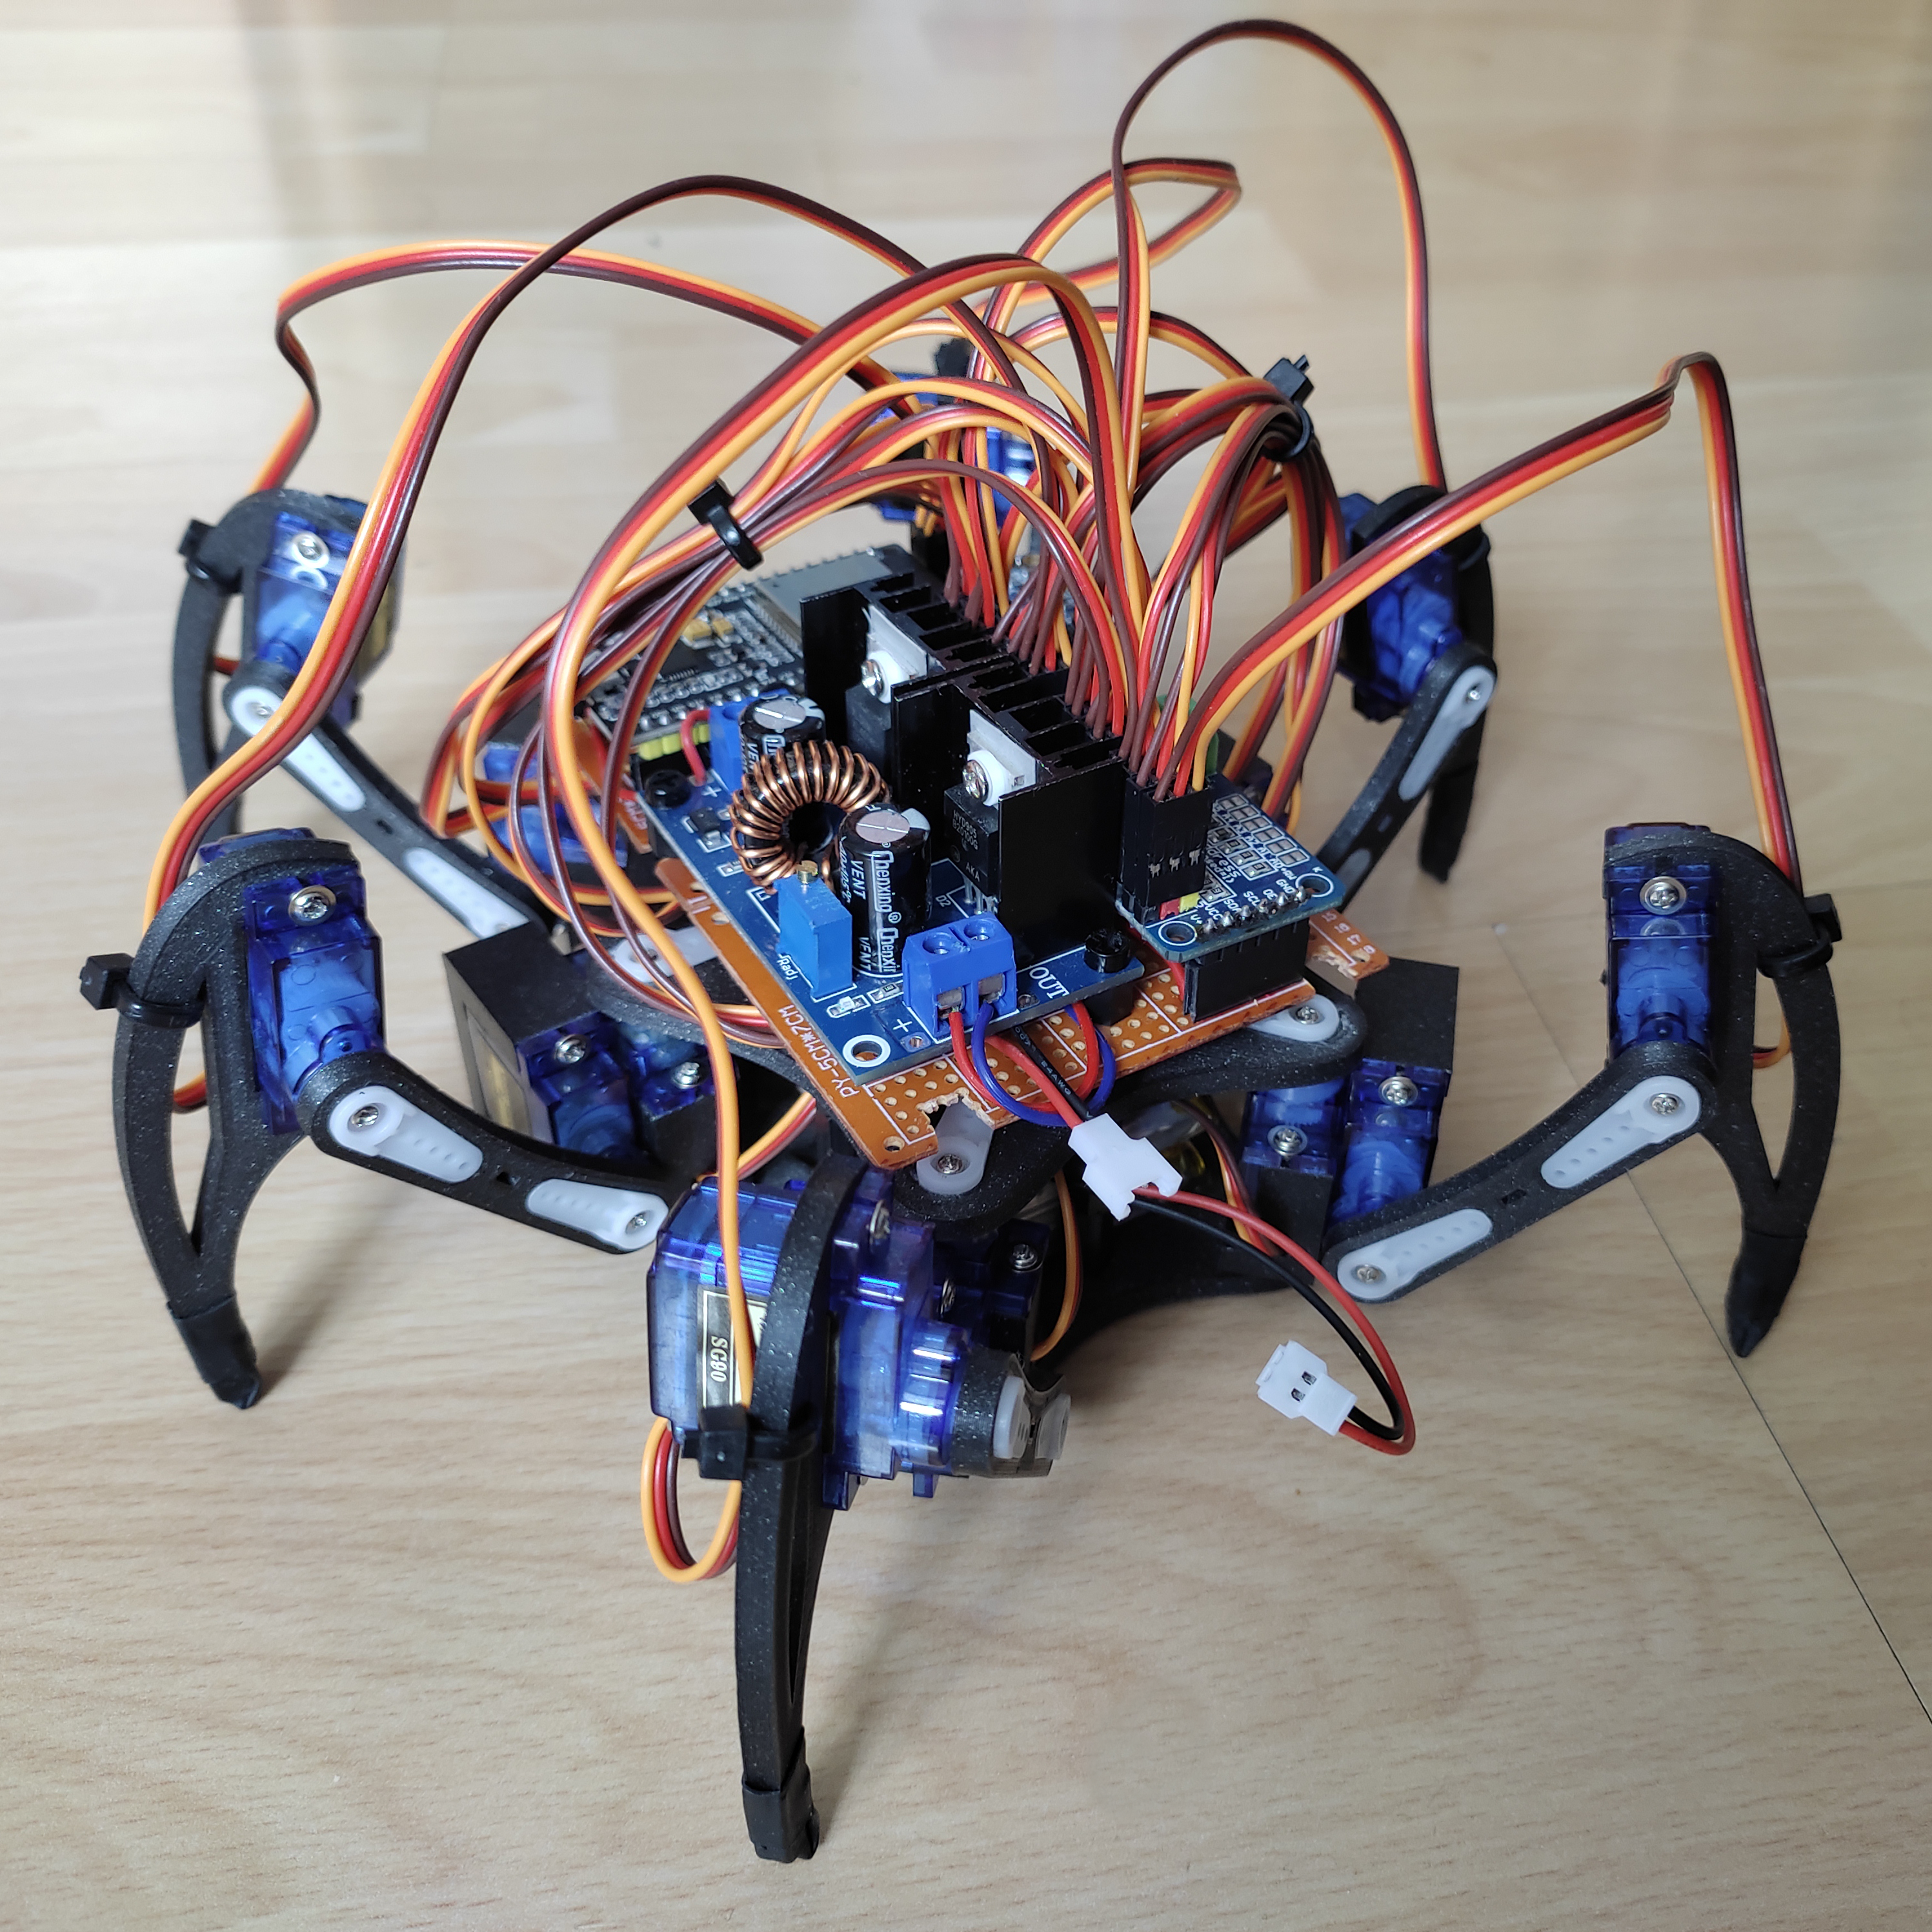
\includegraphics[width=0.7\textwidth]{obrazky-figures/finalrobot.png}
	\caption{Vzhled výsledného robota (celková hmotnost je 550g)}
    \label{finalrobot}
\end{figure}

\subsection*{řídící program robota}
Pro řízení hardwarových částí bylo třeba napsat program pro správné chování celkového robota. Modul ESP32 podporuje spouštění aplikací napsaných v různých programovacích jazycích jako je například C, C++ nebo Micropython. Kvůli zkušenostem a široké podpoře knihoven pro hardware jsem se rozhodl pro jazyk C++ v kombinaci s vývojovým prostředím Arduino IDE. Toto vývojové prostředí je kromě textového editoru vybaveno i nástroji pro správu různých vývojových desek nebo přímý překlad a nahrávání programu na zvolenou vývojovou desku. Arduino IDE také disponuje sériovým monitorem vhodným pro poskytování zpětné vazby při ladění programu. Při použití Arduino IDE musí mít každý napsaný program minimálně dvě funkce: \texttt{void setup()} -- probíhá pouze jednou po spuštění kódu na desce, a \texttt{void loop()} -- smyčka, která běží neustále, dokud nedojde k přerušení běhu programu například restartováním nebo nahráním nového kódu.


\subsubsection*{Inicializace a hlavní smyčka programu}
Hlavní soubor programu obsahuje v první řadě definice používaných proměnných, objektů a některých funkcí. Po spuštění programu je zahájena komunikace s PWM deskou a inicializace serv včetně upřesnění jejich středové polohy. Pro obnovování polohy serv se~na~jádře 1 procesoru vytvoří task (vlákno/úloha) \texttt{TaskRefresh} s vyšší prioritou. Task běží na~samostatném jádře a zaručuje synchronizovaný pohyb všech 18ti serv, což je pro koordinovaný pohyb robota klíčové. Na druhém jádře s identifikátorem 0 probíhá hlavní smyčka programu společně s obsluhou WiFi komunikace.

Hlavní smyčka je složena ze dvou částí. V první části se zpracovávají data, která vysílá uživatelská aplikace prostřednictvím WiFi, a přijaté hodnoty se přiřadí odpovídajícím proměnným. Druhou částí je stavový automat, jehož přechody mezi jednotlivými stavy jsou určovány těmito řídícími proměnnými. Po zapnutí a inicializaci se robot nachází ve stavu \texttt{Sitting}. Jakmile je uživatelem přepnuta poloha robota, dostává se do stavu \texttt{Standing}. \texttt{Standing} se dá považovat za hlavní stav robota, protože je v něm možné měnit výšku a~typ chůze robota. Zvolením směru chůze nebo otáčení přechází robot do příslušného stavu - \texttt{Walking} nebo \texttt{Rotating}. Robot se pohybuje a otáčí podle vybraného typu chůze a výšky. Po~zastavení otáčení nebo chůze je robot zastaven a probíhá úprava jeho končetin do výchozích poloh. Robot je nyní v hlavním stavu \texttt{Standing}.

\begin{figure}[hbt]
	\centering
	\includegraphics[width=0.7\textwidth]{obrazky-figures/HexStateMachine.png}
	\caption{Stavový automat ovládání robota}
    \label{statemachine}
\end{figure}

V kódu jsou použity následující externí knihovny: \texttt{Adafruit\_PWMServoDriver.h} - slouží pro řízení desky s řadičem PCA9685; \texttt{WiFi.h} a \texttt{WifiAP.h} - díky těmto knihovnám lze snadno implementovat WiFi komunikaci a nastavit mód WiFi na přístupový bod.

\subsubsection*{Třída pro práci se servy}
Třída \texttt{MyServo} je základním stavebním kamenem programu robota. Díky této třídě lze serva jednoduše ovládat. Serva se zde řídí pomocí generovaných signálů PWM. Pro odpovídající úhel je vypočítána střída, jež se aplikuje na odpovídající kanál PWM.

Pro plynulost pohybů robota obsahuje tato třída frontu, kde je po dvojicích ukládána požadovaná pozice serva a doba, za kterou má být tato pozice dosažena. To je důležité zejména při implementaci algoritmů, kdy se při jednom kroku robota nastavuje více poloh serva. 

Ovšem nejdůležitější a také klíčovou funkcí pro synchronizovaný pohyb robota je funkce \texttt{Refresh()}. Ve funkci \texttt{Refresh} dochází k aktualizaci polohy serva tak, aby bylo přesně za~daný čas dosaženo požadované polohy. Jestliže dojde k přesažení tohoto času, je servu přímo nastavena požadovaná poloha a z fronty je načtena nová poloha společně s novou dobou trvání. Přesný úhel odpovídající danému času je vypočítáván pomocí vzorce:
$$angle = angle_{prev} + (angle_{des} - angle_{prev}) * \frac{time_{curr} - time_{start}}{duration}$$

\noindent kde $angle$ je výsledný úhel, $angle_{prev}$ -- předchozí (současný) úhel, $angle_{des}$ -- požadovaný úhel, $time_{curr}$ -- aktuální čas, $time_{start}$ -- čas začátku pohybu pro aktuální požadovaný úhel a $duration$ -- doba za kterou má být dosaženo požadovaného úhlu.


\subsubsection*{Implementace končetiny}
Samotná končetina se skládá ze tří serv a její hlavní funkcí je nastavení polohy špičky končetiny pomocí XYZ souřadnic, k čemuž byla použita inverzní kinematika. Díky této funkci lze s končetinami snadno pracovat.

Při zastavení chůze/otáčení robota je aktuální poloha končetiny dopočítána přímou kinematikou a následně již inverzní kinematikou položena na zem. To je z důvodu bezpečného položení zdvižené končetiny na zem.

\subsubsection*{Pohybové algoritmy robota}
\texttt{Hexapod} je složen z šesti končetin a ukládá si aktuální stav do proměnné. Tato třída obsahuje všechny potřebné pohybové algoritmy pro různé typy chůze. Implementovány byly algoritmy pro pohyb i otáčení v režimu tripedální, ``4+2'' a vlnové chůze. Pro každou chůzi je~napsána funkce pro přípravu kroku, kvůli plynulému přechodu z klidového stavu a funkce pro samotný krok.

Algoritmy pro různé typy chůze se liší pouze v časování jednotlivých končetin a době, po~kterou se končetiny dotýkají země. Typický tvar pohybu zdvihání a pokládání jedné končetiny (na obrázku \ref{legmovement}) při libovolném algoritmu zůstává stejný. Díky časování jednotlivých segmentů pohybu bylo dosaženo přirozenějšího pohybu robota.

\begin{figure}[hbt]
	\centering
	\includegraphics[width=0.75\textwidth]{obrazky-figures/legmovement.png}
	\caption{Časování a tvar pohybu špičky končetiny ve svislé ose pro různé typy chůze}
    \label{legmovement}
\end{figure}


\section{Mobilní aplikace pro dálkové ovládání robota}
Robota lze dálkově ovládat prostřednictvím snadno použitelné uživatelské aplikace. Aplikace byla vytvořena pro telefony s verzí operačního systému Android 6.0 a novější. Pro~vývoj aplikace jsem použil vývojové prostředí Android Studio, a programovací jazyk, ve kterém byla aplikace napsána je Java. Vývoj mobilní aplikace sestává ze dvou základních částí. Jednou částí je uživatelské rozhraní a druhou samotná implementace funkčnosti logiky aplikace. Při vývoji aplikace pro Android je hlavní částí programu tzv. activity, bez níž by aplikace nešla spustit. Activity je prezenční vrstvou aplikace. Každá activity má daný svůj životní cyklus (obrázek \ref{activity}) a má k dispozici několik callbacků. Povinná je implementace callbacku onCreate(), kde se vytváří základní logika aplikace (například propojení prvků GUI s objekty v kódu).

\begin{figure}[hbt]
	\centering
	\includegraphics[width=0.65\textwidth]{obrazky-figures/activity_lifecycle.png}
	\caption[activity]{Zjednodušená ilustrace životního cyklu Activity\footnotemark}
	\label{activity}
\end{figure}
\footnotetext{Obrázek převzat z: https://www.oreilly.com/library/view/android-programming-the/9780135257555/ch03s02.html}


\subsection*{Uživatelské rozhraní}
Uživatelské rozhraní tvoří jedna hlavní obrazovka se všemi potřebnými ovládacími prvky. Největší změnou proti původnímu návrhu je vertikální orientace obrazovky. Také bylo odstraněno tlačítko pro manuální připojování, protože aplikace se na určitý síťový port připojuje automaticky, pokud je telefon připojen k WiFi. O stavu úspěšného připojení, případně odpojení je uživatel informován pomocí textu \texttt{Connected/Disconnected}. Pro řízení pohybu robota byly nejprve navrženy šipky do osmi směrů. Tento způsob ovládání byl nahrazen všesměrovým virtuálním joystickem, obsaženým v externí knihovně\footnote{Knihovna je dostupná z: https://github.com/controlwear/virtual-joystick-android}. Díky joysticku lze robotovi určit libovolný směr chůze a plynule jej měnit.

Ve finální verzi uživatelského rozhraní (obr.~\ref{appgui}) přibylo jedno tlačítko na složení/rozložení robota -- přepínání stavu robota mezi stavy \texttt{Sitting} a \texttt{Standing}. Tlačítky ve skupině \texttt{Height} lze přepínat výšku chůze robota, s čímž se zároveň mění i jeho rychlost -- pokud je robot nízko, končetiny nemusí být zvedány do velké výšky a proto se mohou pohybovat rychleji. Naopak pokud je robot vysoko, dělá vyšší kroky a pohybuje se pomaleji. Pro~přepínání režimů chůze robota slouží tlačítka ve skupině \texttt{Gait}. Zde je na výběr mezi tripedální chůzí ``3+3'', chůzí ``4+2'' a vlnovou chůzí ``5+1''. Robota lze pak otáčet doleva nebo doprava za pomocí příslušné šipky znázorňující rotaci.

\begin{figure}[hbt]
	\centering
	\includegraphics[width=0.35\textwidth]{obrazky-figures/appgui.jpg}
	\caption{Grafické uživatelské rozhraní aplikace}
    \label{appgui}
\end{figure}

\subsection*{Backend aplikace}
V rámci životního cyklu activity je v aplikaci implementován pouze callback \texttt{onCreate()} a \texttt{onStart()}. V callbacku \texttt{onCreate()} probíhá přiřazení akcí provedených při stisku tlačítek/pohybu joysticku. Aby při pohybu joystickem nedocházelo k pohybu robota ve špatném směru, je úhel joysticku zaznamenáván, až pokud je jeho hodnota za polovinou maximálního rozsahu. Při každém stisku tlačítka/pohybu joystickem jsou pomocí socketu odesílána data nesoucí hodnoty všech ovládacích prvků. Tímto se zajistila aktualizace změněných hodnot. Tyto hodnoty jsou odesílány prostřednictvím TCP socketu na řídící desku robota.

Callback \texttt{onStart()} spouští úlohu, která běží periodicky a odesílá charakter pro kontrolu aktivního spojení. Program na modulu ESP32 kontroluje, zda byl přijat tento charakter a tím pádem přesně určuje, zda je spojení s uživatelem aktivní.


\pagebreak

\section{Dosažené cíle a možná zlepšení}
\label{secResults}
Určení, zda bylo dosaženo cílů vytyčených v části \ref{specs}, se věnuje tato část. Úvodní zadání jsem splnil, výsledkem práce je tedy šestinohý robot s 18 stupni volnosti a je možno jej dálkově ovládat pomocí mobilní aplikace. Kromě tohoto bylo třeba porovnat a ověřit předpokládané vlastnosti robota:

\begin{itemize}
    \item \textbf{Jednoduchá konstrukce, výměna dílů} -- 3D model robota obsahuje pouze nezbytné části a nedisponuje žádnými složitými díly. Serva byla do dílu připevněna pomocí šroubů, tudíž lze v případě poškození vyměnit jak serva, tak tištěné díly. Co~se~týče elektronických částí, jednotlivé moduly jsou zasazeny v dutinkách, a tak jdou snadno vyměnit kus za kus. Baterie lze vytáhnout po odšroubování spodní části těla robota. Tento bod považuji za splněný.
    \item \textbf{Cenová dostupnost} -- celková cena použitých dílů je \textasciitilde\$60, což je zlomek ceny, za kterou se dají pořídit komerční řešení obdobných robotů.
    \item \textbf{Všesměrová chůze ``3+3''} -- robot je schopný se pohybovat libovolným směrem v~režimu tripedální chůze, přičemž lze tento směr plynule měnit při pohybu robota.
    \item \textbf{Bezdrátové ovládání} -- robota lze dálkově ovládat pomocí aplikace z libovolného mobilního telefonu s operačním systémem Android ve verzi 6.0 a vyšší. Uživatelské rozhraní obsahuje pouze nutné prvky k ovládání a jednoduše se používá.
    \item \textbf{Bateriové napájení} -- pro napájení byly použity 2 LiPol baterie s dostatečnou kapacitou pro dlouhý provoz robota. Baterie byly zapojeny sériově pomocí redukce. Při~nabíjení baterií je nutné tuto redukci odpojit a nabíjet každou baterii zvlášť.
    \item \textbf{Otáčení robota na místě} -- robot se umí otáčet v obou směrech při různých režimech chůze v libovolně zvolené výšce.
    \item \textbf{Změna výšky chůze} -- uživatel si může zvolit jednu ze tří možností výšky chůze robota. Konkrétní vzdálenosti mezi zemí a spodní částí těla robota jsou $15mm$, $30mm$ a $50mm$.
    \item \textbf{Varianty chůze ``4+2'' a ``5+1''} -- obě varianty byly implementovány a uživatel může přepínat mezi třemi režimy chůze.
    \item \textbf{Pohyb v různých terénech} -- robot je schopen se pohybovat po více typech terénu, více v sekci testování \ref{tests}.
\end{itemize}

Možného zlepšení by mohlo být dosaženo použitím kvalitnějších serv, protože použitá serva mají nepatrnou vůli na páce. Kvůli tomuto dochází při chůzi k třasu některých zdvižených končetin. Nicméně tato vlastnost nemá žádný vliv na funcionalitu robota. Také zvolený typ baterií je mírným omezením kvůli jejich nízkému počtu C. Výměnou za silnější baterie a mírnými úpravami kódu by bylo dosaženo svižnějšího a rychlejšího pohybu robota.

Nejvýzamnějšího zlepšení je možné docílit vybavením všech končetin senzory došlapu a~přepracováním kódu. Tímto by se eliminovaly případy, kdy některé končetiny zůstávají ve~vzduchu jakmile se robot nachází na nerovném povrchu.

\section{Testování robota}
\label{tests}
Za účelem ověření klíčových vlastností robota jsem sestavil a realizoval testy. Nejvíce testovanou vlastností byla průchodnost rozdílnými terény při různém nastavení robota.

\subsection*{Pohyb v různých terénech}
Tato sada experimentů testuje pohybové vlastnosti robota v různých terénech. Při testech byly vyzkoušeny různé kombinace nastavení výšky robota a typu chůze.

\begin{itemize}
    \item \textbf{Chůze po hladkém povrchu (podlaha) -- Úspěch} -- robot se bez problémů dokáže pohybovat a otáčet v libovolném směru při každém nastavení výšky i typu chůze.
    \item \textbf{Chůze po hrubém povrchu (nízký koberec) -- Úspěch} -- pohyb robota je stejně bezproblémový jako na hladkém povrchu.
    \item \textbf{Pohyb v členitém terénu (rozsypané lego kostky) -- Úspěch} -- při nastavení nejnižší výšky nebyl robot schopen zdvihnout končetiny dostatečně vysoko, aby mohl překročit kostky. Robot se začal správně pohybovat až při nastavení nejvyšší polohy. V této poloze byly poté testovány jednotlivé typy chůze. Při tripedální chůzi se robot propadal mezi kostky a převažoval se do stran -- pohyboval se velmi obtížně. Po~přepnutí na chůzi ``4+2'' se robot dokázal pohybovat bez větších problémů. Nejlepšího výsledku bylo dosaženo v kombinaci nejvyšší polohy společně s vlnovou chůzí. V tomto režimu se robot dokázal po kostkách bez problémů pohybovat.
    \item \textbf{Chůze po měkkém povrchu (postel) -- Úspěch} -- s nejnižší polohou se robot pohyboval dost problematicky nezávisle na typu chůze. Nicméně při středním nastavení výšky byl již schopen bezproblémové chůze i otáčení libovolného typu.
    \item \textbf{Pohyb v nízké trávě \textasciitilde3cm -- Úspěch} -- s nejnižší polohou byl robot plnou vahou opřen o trávu a tak se prakticky nehnul z místa za použití libovolného režimu chůze. Po zvýšení na střední hodnotu se začal mírně pohybovat, nicméně byl stále opřen o~trávu. Až při zvolení nejvyšší polohy byl robot schopen správného pohybu při všech typech chůze.
    \item \textbf{Pohyb ve svahovitém terénu \textasciitilde25° (tráva) -- Neúspěch} -- kvůli výšce trávy musela být vybrána nejvyšší poloha robota. Bohužel při pokusu o chůzi se robot převrátil kvůli vysokému těžišti.
    \item \textbf{Pohyb ve svahovitém terénu \textasciitilde25° (beton) -- Úspěch} -- robot sice jevil mírné problémy při stoupání do svahu, nicméně byl schopen jej vylézt s nejnižším i středním nastavením výšky ve všech režimech chůze. Nejvyšší poloha nebyla testována, protože hrozilo možné převrácení robota.
\end{itemize}

Z těchto testů vyplývá, že robot je bez větších potíží schopen pohybu v různě členitých terénech, které se příliš nesvažují. Tripedální chůze je ideální především k pohybu v~rovnějších terénech, ``4+2'' a vlnová chůze umožňují robotovi překonávání náročnějších a~členitých terénů. Robot není při současné implementaci vhodný do svažujících se povrchů.


\subsection*{Testy výdrže robota}
Tyto experimenty jsou zaměřeny na vlastnosti zpracování robota, odolnost jeho konstrukce a elektroniky. Nicméně kvůli jejich povaze nebyla většina testů realizována, aby nedošlo ke~zničení robota. Minimálně následující testy je nutné provést pro zajištění kvality robota před případným uvedením na trh.

\begin{itemize}
    \item \textbf{Test nosnosti robota} -- tento test by měl prověřit sílu robota a jak těžké těleso dokáže unést. Kvůli konstrukci robota a absenci nákladního prostoru nebyla testována chůze se zátěží. Test tedy proběhl experimentem, zda se robot s různě těžkými tělesy dokáže postavit a je schopen měnit svou výšku. Nejtěžší těleso, se kterým se robot zvládl postavit a změnit svou výšku, mělo váhu 460 gramů. 
    \item \textbf{Pevnost konstrukce} -- zde by měly být jednotlivé díly konstrukce podrobeny zátěžovým testům a měřen tlak/zátěž potřebný k jejich zničení. Tento test nebyl realizován z důvodu zničení robota.
    \item \textbf{Opotřebení serv} -- protože serva jsou složena z mechanických prvků, může opakovaným používáním dojít k jejich opotřebení a poruše. Z důvodu omezeného času této práce nebyla možnost test realizovat.
    \item \textbf{Opotřebení baterií} -- u každé baterie časem dochází k její degradaci a poklesu celkové kapacity. Ze stejných důvodů jako v předchozím případě nebyl tento test realizován.
    \item \textbf{Kvalita elektroniky} -- použité elektronické části nemám zcela vyzkoušené, a tak mohou z různých důvodů po delším čase přestat fungovat. Celkovou životnost jsem také z důvodu omezeného času této práce nemohl testovat.
\end{itemize}


%=========================== Závěr
\chapter{Závěr}
\label{zaver}
V této práci bylo cílem navrhnout a vytvořit robota sestrojeného z modelářských serv. Cíl byl splněn a výsledkem je dálkově ovládaný šestinohý robot, připomínající robotického brouka.

Nastudoval jsem princip činnosti modelářských serv, způsoby jejich řízení a vlastnosti. Na záladě těchto znalostí a dostupných technologiích byl navržen strojek s modelářskými servy, konkrétě se jednalo o šestinohého kráčejícího robota. Pro tento návrh byly zvoleny vhodné elektronické komponenty a vytvořeny mechanické díly. Následně proběhla realizace tohoto návrhu, přičemž byl robot doplněn o dálkové ovládání v podobě mobilní aplikace. V implementaci pohybu robota bylo využito inverzní kinematiky pro přirozený pohyb končetin. Po dokončení sestavení robota, implementace řídícího programu a ovládací aplikace jsem shrnul cíle, kterých bylo dosaženo a prodiskutoval možná zlepšení. Robot byl v závěru podroben několika experimentům, které testovaly zejména průchodnost rozdílnými terény.

Ke stavbě robota bylo použito celkem 18 serv, tím pádem má k dispozici 18 stupňů volnosti. Nákupní cena elektroniky a jiných součástek byla odhadnuta na \$60, přičemž 3D tisk dílů jsem neplatil. Robot má implementovány 3 režimy chůze, a je možné zvolit jednu ze tří výškových poloh robota.

Práce mi dala nové zkušenosti s ovládáním a synchronizací většího množství serv, která se pohybují nezávisle na sobě. Kromě toho jsem si vyzkoušel aplikaci inverzní i dopředné kinematiky na konkrétním příkladě.

V práci by bylo možné pokračovat opatřením končetin robota vhodnými senzory pro určení, zda se dotýkají země, a přizpůsobením 3D modelu konkrétního dílu. Mimo to by mohl být robot vybaven výkonnější řídící deskou a doplněn kamerou, případně dalšími diagnostickými senzory (například pro měření vlhkosti, tlaku, teploty a jiných veličin v~nepřístupných prostorách).

%===============================================================================
